\documentclass[12pt,a4paper,twoside,openright]{report}


\usepackage{graphics}       % Graphics commands
\usepackage{wrapfig}        % Wrapping text around figures
\usepackage{epsfig}         % Embed encapsulated postscript
\usepackage{rotating}       % Extra graphics rotation
\usepackage{longtable}      % Page breaks within tables
\usepackage{supertabular}   % Page breaks within tables
\usepackage{multicol}       % Allows table cells to span cols
\usepackage{multirow}       % Allows table cells to span rows
\usepackage{texnames}       % Macros for common tex names

\usepackage{listings}       % Source code listings
\usepackage{array}          % Array environment
\usepackage{url}            % URL formatting
\usepackage{amsmath}        % American Mathematical Society
\usepackage{amssymb}        % Maths symbols
\usepackage{amsthm}         % Theorems
%\usepackage{mathpartir}     % Proofs and inference rules
\usepackage{verbatim}       % Verbatim blocks
\usepackage{ifthen}         % Conditional processing in tex
\usepackage{xcolor}         % X11 colour names
\usepackage{ulem}

\usepackage{tikz}
\usetikzlibrary{arrows, automata}
\usepackage[margin=25mm]{geometry}
\usetikzlibrary{shapes,fit,calc,positioning}

\usepackage{float}

\usepackage{biblatex}
\addbibresource{dissertation.bib}

\usepackage{pgfplots}
\pgfplotsset{compat=1.12}

\usepackage[toc,page]{appendix}

\usepackage{placeins}

\usepackage{pdfpages}

%\setlength{\oddsidemargin}{-20pt}
%\setlength{\evensidemargin}{-20pt}
%\setlength{\topmargin}{-65pt}
%\setlength{\textwidth}{475pt}
%\setlength{\marginparwidth}{100pt}
%\setlength{\textheight}{720pt}

\setlength{\parindent}{0em}
\addtolength{\parskip}{1ex}
\title{
{\Large Computer Science Tripos -- Part II -- Project Proposal}\\
\vspace{1em}
Incentivising distributed file storage using blockchain contracts.}
\author{Ben Ramchandani \\ bjr39@cam.ac.uk \\ St. Catharine's College}
\date{\today}


\begin{document}
\begin{titlepage}
\hfill \textbf{\Large Ben Ramchandani}
\vspace{10em}
\begin{center}
{\huge \bfseries Incentivising distributed file storage using blockchain contracts}\\
\vspace{2em}
{\Large Computer Science Tripos -- Part II}\\
\vspace{2em}
{\Large St. Catharine's College}\\
\vspace{2em}
{\Large \today}
\end{center}
\end{titlepage}

\chapter*{Proforma}

{
\begin{tabular}{ll}
Name:               & \bf Ben Ramchandani\\
College:            & \bf St. Catharine's College\\
Project Title:      & \bf Incentivising distributed file storage using blockchain contracts\\
Examination:        & \bf Computer Science Tripos -- Part II, July ****  \\
Word Count:         & \bf ****\footnotemark[1]\\
Project Originator: & Ben Ramchandani\\
Supervisor:         & John Knox\\ 
\end{tabular}
}
\footnotetext[1]{This word count was computed
by \texttt{detex diss.tex | tr -cd '0-9A-Za-z $\tt\backslash$n' | wc -w}
}
\stepcounter{footnote}

\section*{Original Aims of the Project}


\section*{Work Completed}

All that has been completed appears in this dissertation.

\section*{Special Difficulties}

None.

\section*{Declaration}

I, Ben Ramchandani of St. Catharine's College, being a candidate for Part II of the Computer
Science Tripos, hereby declare
that this dissertation and the work described in it are my own work,
unaided except as may be specified below, and that the dissertation
does not contain material that has already been used to any substantial
extent for a comparable purpose.

\bigskip
\leftline{Signed}

\medskip
\leftline{Date}

\newpage


\tableofcontents

\listoffigures

All figures used have been created by me in \LaTeX, using the \texttt{tikz} package for diagrams and the \texttt{pgfplots} package for graphs.

%%%%%%%%%%%%%%%%%%%%%
\chapter{Introduction}

\section{Overview}

The aim of this project is to create a system which allows you to pay others for storing files on your behalf without requiring a trust relationship or a trusted third party.
I use the a Bitcoin like network, Ethereum, to provide the trustless contract between the two actors.
The main difficulty here is finding a cryptographic protocol that allows someone to prove they have access to a file without sending the whole file to the Ethereum network.

\section{Context and motivation}

The context in which such a payment system would be useful is a Distributed File System (DFS).
Several distributed file systems exist, however there is not usually any incentive to run a node and participate in the network.
An incentive system may help a DFS grow as more people can run nodes.

There are essentially two problems to be solved to create such an incentive system
\begin{itemize}
\item Compensating nodes for sending files to you on request.

\item Compensating nodes for storing files for extended periods.
For example, if you wished to use the DFS as a back up for data, then it is likely you will never request the files you store,
however you still want confidence that the files exist in the network in case you lose your primary copy.
\end{itemize}

The first problem is interesting in itself, and has a possible solution in micro-payment channels over Bitcoin or a similar cryptocurrency,
however it is not discussed here.

This dissertation concerns itself with a possible set of solutions to the second problem.
The problem statement is simple, we wish to pay another node at some fixed point in the future if and only if they our still storing our file.

In a DFS there is not usually any trust between nodes, or a central trusted party, since this would introduce a single point of failure.


\section{Scope of project}

The model for this project is as follows:

At time $T_0$ the file owner and some storing node both have access to a file $F$. The owner wants to pay the storing node
after some time $T_0 + t$ has passed if and only if the storing node still has access to the file.

The following constraints apply to the problem
\begin{itemize}
\item The owner will not pay if they can avoid doing so whist still being confident that the file will be stored
\item The storing node will try to get paid without storing the file if it can do so
\item The owner does not have access to the file after time $T_0$
\item There is no trusted third party, except the Ethereum network
\end{itemize}

Notably I do not consider how the storing node initially gains access to the file, or how the owner could retrieve the file if they wished to.
These problems are considered to be out of scope of the project.
% I do not consider how the file gets to the storing node, or how the file is retrieved.
% The aim is to pay someone if and only if they still have access to a file after a certain period of time.
% The file owner doesn't trust the person storing it and vice-versa.

% Should be secure against
%% The storer deleting the file before the time is up.
%% The user attempting to have the file stored without paying, being able to cancel

\section{Ethereum}

The Bitcoin cryptocurrency, proposed in 2008, allows its users to pay for goods and services using digital money
without relying on a trusted party to mediate the transaction.

Ethereum is another cryptocurrency that extends this idea by also allowing accounts to be controlled by blobs of code.
This allows its users to form financial contracts that are defined concretely in code and enforced automatically by the network.


\section{Original plan}

Figure \ref{project-overview} shows the basic structure of the project as proposed.

\begin{figure}[h]
\centering
\begin{tikzpicture}


\coordinate(O1) at (0,0);
\node[above right=0.5cm and 3.2cm of O1](t0) {$T_0$};
\node[above right=0.5cm and 9.9cm of O1](t1) {$T_0 + t$};

\node[below right=0cm of O1](s) {Storage node};
\node[below = 3 cm of s](b) {Ethereum};
\node[below = 3 cm of b](o) {File owner};

\node[below right=-0.2cm and 3cm of O1,draw, minimum width=1cm,minimum height=1cm,fill=white](sf) {$F$};
\node[below right=7cm and 3cm of O1,draw, minimum width=1cm,minimum height=1cm,fill=white](of) {$F$};

\node[below right=2.5cm and 3cm of O1,draw, minimum width=2.2cm,minimum height=3cm,fill=white](c) {Contract};

\node[below right=-0.2cm and 10cm of O1,draw, minimum width=1cm,minimum height=1cm,fill=white](sft) {$F$};
\node[below right=2.5cm and 10cm of O1,draw, minimum width=2.2cm,minimum height=3cm,fill=white](ct) {Contract};
\node[below right=-0.2cm and 11.2cm of O1,minimum width=1cm,minimum height=1cm,fill=white](smoneyt) {\$};

\draw[->, very thick] (of) -- node[left] {Upload} node[right] {($X$ Ether)} (c);
\draw[->, thick, dashed] (t0) -- (t1);
\draw[->, thick, dashed] (c) -- (ct);
\draw[->, thick, dashed] (sf) -- (sft);
\draw[->, very thick] (sft) -- node[left, align=center] {Submit proof of\\ retrievability for $F$} (ct);
\draw[->, very thick] (ct) -- node[right, align=center] {Pays for valid proof\\($X$ Ether)} (smoneyt);
\end{tikzpicture}
\caption[Project overview]{An overview of the proposed structure of the project.}
\label{project-overview}
\end{figure}

At time $T_0$ the file owner places a contract on the Ethereum blockchain that contains some information about the file $F$.
At time $T_0 + t$ the storing node submits a proof that they still have access to the file and if the proof is correct they will be paid.

The main technical challenge in this set-up is forming a proof of retrievability that is both
\begin{itemize}
\item public -- all information in the contract is public and the owner does not need to provide any new information
\item compact -- uploading the whole file to the Ethereum network would be prohibitively expensive
\end{itemize}

\section{Inspiration for proposal}

I first saw the idea for using Ethereum contracts to fund off chain file storage in the Ethereum Whitepaper \cite{eth-whitepaper}.
In this report I implement and expand on this idea, looking at different implementations and any limitations of Ethereum I encounter.

%\section{Nomenclature}




\chapter{Preparation}

\section{Starting point}

All of the code submitted has been written during the project.

I had some understanding of Bitcoin and Ethereum from researching it as a possible project area over the summer break.
I had not used the language Solidity, in which the Ethereum contract is written before starting the project.

\section{Original aims of preparation stage}

I had four main aims going into the preparation stage.
\begin{itemize}
\item Background reading.

My understanding of Ethereum and other cryptocurrencies was limited going into the project, so I wanted to
take some time to read up on the area. I also wanted to find out if anything similar to what I was planning
had been implemented before.

\item Proofs of retrievability.

Perhaps the most academically interesting part of this project is how to prove one has access to a file
under the constraints that apply to Ethereum contracts.
There is some literature on the subject (of proofs of retrievability in general, not specific to Ethereum),
which I only had time to investigate briefly before submitting the project proposal.
I planned to spend some time reading and understanding this.

\item Solidity.

Solidity is a programming language that compiles Ethereum contracts.
I plan to write the contract for this project in Solidity, so I needed to learn it.

\item Design and planning.

I wanted to plan out in detail the interface between the contract and the proof generation system,
so I could start developing them knowing they will work together.


\end{itemize}


\section{Background}

I have included relevant background information about Ethereum in an attempt to make this report self sufficient.
This information is primarily drawn from the original Bitcoin paper\cite{bitcoin-whitepaper} and the Ethereum Whitepaper\cite{eth-whitepaper}.

\subsection{Cryptographic hash functions} \label{crypto-hash}

We take the definition used by Merkle \cite{merkle-thesis}.

A cryptographic hash function is a function $h: \{0, 1\}^* \to \{0, 1\}^N$ for some fixed output size $N$.

It has the properties that
\begin{itemize}
\item Given any $x$ it is easy to compute $h(x)$.
\item Given $h(x)$ it is computationally infeasible to find $x$.
\item Given any $x$ it is computationally infeasible to find an $x'$ such that $x \neq x'$ and $h(x) = h(x')$.
\end{itemize}

We take the second property to also cover the case where you are given $x$ and $h(x || y)$ (here $||$ denotes concatenation), in that it is computationally infeasible to find $y$.
Similarly for $h(y || x)$.



\subsection{The Blockchain}

A blockchain is a distributed database that holds its data in an ordered list of records, called blocks.
Each block has, at a minimum, a payload and the hash of the previous block.
In this way, given any block it is possible to use the hashes to trace back a chain of blocks to some initial block.
Provided a secure cryptographic hash function is used, this chain is tamper resistant in that altering any block will break this chain.

\begin{figure}[h]
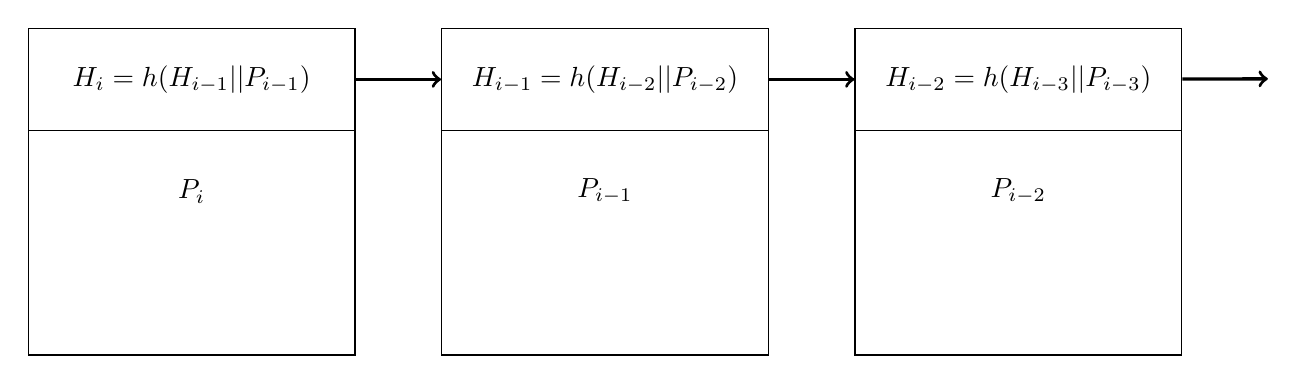
\begin{tikzpicture}


\coordinate(O1) at (0,0);
\node[below right=0cm of O1,draw, minimum width=4.15cm,minimum height=4.15cm,fill=white](block1) {$P_i$};
\node[below right=0cm of O1,draw, minimum width=4.15cm,minimum height=1.3cm,fill=white](hash1) {$H_i = h(H_{i-1} || P_{i-1})$};


\coordinate(O1) at (5.25,0);
\node[below right=0cm of O1,draw, minimum width=4.15cm,minimum height=4.15cm,fill=white](block2) {$P_{i-1}$};
\node[below right=0cm of O1,draw, minimum width=4.15cm,minimum height=1.3cm,fill=white](hash2) {$H_{i-1} = h(H_{i-2} || P_{i-2})$};

\coordinate(O1) at (10.5,0);
\node[below right=0cm of O1,draw, minimum width=4.15cm,minimum height=4.15cm,fill=white](block3) {$P_{i-2}$};
\node[below right=0cm of O1,draw, minimum width=4.15cm,minimum height=1.3cm,fill=white](hash3) {$H_{i-2} = h(H_{i-3} || P_{i-3})$};

\draw[->, very thick] (hash1) -- (hash2);
\draw[->, very thick] (hash2) -- (hash3);
\draw[->, very thick] (hash3) -- (15.75, -0.65);
\end{tikzpicture}
\caption[A simple blockchain]{A graphical representation of a Blockchain.
Each block consists of a payload $P_i$ and a hash $H_i$ of the previous block.
Here $h$ is the hash function and $||$ denotes concatenation.}
\label{Blockchain}
\end{figure}

\subsection{Bitcoin}

The idea for Bitcoin first appeared in 2008 with a paper by the (still unidentified) Satoshi Nakamoto \cite{bitcoin-whitepaper}.
It is based on a continuously growing blockchain, with transactions stored as payloads.
Creating a new block requires solving a computationally difficult problem, however the person who creates the block is rewarded with Bitcoins.
The longest valid chain of blocks is considered to be the correct one and this allows a distributed consensus to be formed,
giving an order to transactions.

The first Bitcoin client was released in 2009, again by Satoshi Nakamoto.
Since then it has been maintained by the community and several other similar cryptocurrencies have emerged.

% More techincal.

Each user in Bitcoin has a public/private key-pair, with the public key also acting as an address.
Coins may be sent to any address, but spending coins requires the signing of the transaction with the user's private key.

Bitcoins are created when new blocks are minted by `miners',
in the form of a special transaction awarding Bitcoins to the miner (or any other address of their choosing).

All other transactions consist of a list of input coins, along with proofs of ownership (normally just a digital signature)
and a list of output coins, along with a description of what is required to spend them in the future (again normally a digital signature from some address).
The transaction is then signed with the user's private key and broadcast to the network.
Each node in the network verifies that each of the input coins is valid (the unlocking proof is valid
and the coin has not already been spent), that the signature is valid for that address and that the total value of the inputs is at least that of the outputs.
The transaction will then be added to the next block, which each node verifies before beginning work on further blocks.


\subsection{Ethereum}


Ethereum is another cryptocurrency, initially propsed in late 2013 \cite{eth-whitepaper}.
it is based on the same ideas as Bitcoin, but extended with a Turing complete language
embedded in the protocol.
There are also several other changes primarily intended to improve performance, however they are not relevant here.
It's base currency is known as Ether.

An address controlled by a blob of code is referred to as a \textit{smart contract}.
The contract analogy holds in the sense that the contract cannot be modified or removed by
its owner or any other party, except in ways defined in the contract itself.
As such, if you put money (Ether) into a smart contract, you are bound to its terms.

The contract code is stored on the blockchain and whenever a transaction is sent to its address the code is executed,
and may in turn call other contracts or send Ether to other addresses.
In this way the code becomes part of the block verification process run by all nodes in the network.

To prevent denial of service attacks each step of execution costs money to the transaction sender.
Any transaction intended for a contract should include some amount of `gas', which must be paid for in Ether.
The contract code is then executed until it either terminates or runs out of gas.

\subsection{The EVM}

%Learning a new language counts for something, talk about solidity.

I'll refer to the language used by Ethereum as EVM (Ethereum Virtual Machine) code.
It is a stack based bytecode, with a word size of 256 bits (the output size of the hash function used by Ethereum, and the size of an address).
Contracts can have multiple entry points and may receive arguments as binary data.

When executing contracts have access to three types of storage

\begin{itemize}
\item the stack

For local variables, this is cheap to access (in terms of gas cost).
It does not persist between calls to the contract.

\item memory

Analogous to the a heap in a normal execution environment, larger structures and arrays can be stored here.
It is slightly more expensive to access.
It does not persist between calls to the contract.

\item storage

Permanent storage on the blockchain.
In comparison this is very expensive to access, but allows data to persist between contract invocations.
\end{itemize}

All data sent to or held by a contract is public knowledge as it is shared between all nodes.
As such private data must be stored off chain or encrypted before sending.
The hashes of the last 256 blockchain blocks are available to contracts in the EVM, not including that of the current block (since the block hash depends on the content of the block).

Full detail on Ethereum and the EVM, including opcodes and associated gas costs can be found in the Ethereum Yellow Paper \cite{eth-yellowpaper}.

\subsection{Relevant limitations of Ethereum}

\begin{itemize}
\item No external source of randomness can be used as the computation must be deterministic,
however block hashes may be used for this purpose and cannot be predetermined.

\item All data sent to or held by a contract is public knowledge as it is shared between all nodes.

\item Storing data on the blockchain is expensive (stored by all nodes).
For this reason we cannot simply store the whole file on the blockchain.

\item Sending data to the blockchain is expensive (stored by all nodes).
As such we cannot send the whole file to the blockchain.

\item Extensive computations are expensive.
%See section \ref{ext-ecc}.

\item Block hashes are only available for the last 256 blocks.
There are ways to get round this, but it will not be necessary here**.
\end{itemize}


%Advantages:

% Contracts cannot be withdrawn (unless in code)


%This should be somewhere else
%\subsection{RSA}
%
%Let $e$, $p$ and $q$ be large primes.
%Let $N = p \cdot q$.
%Find $d$ such that $e d \equiv 1 \mod (p-1)(q-1)$.
%
%Now we have $(m^e)^d \equiv m \mod N$ for all $m \in \mathbb{N}_N$.
%Given $e$ and $N$ it is hard to find $d$ unless $p$ and $q$ are known as well.
%This therefore forms a public key encryption system.
%
%Notice that $(m_1^e \cdot m_2^e)^d = \left((m_1 \cdot m_2)^e\right)^d \equiv m_1 \cdot m_2 \mod N$, so we can perform multiplication on
%encrypted messages $m^e \mod N$.
%Similarly $\left(\left(m^e\right)^x\right)^d = \left(\left(m^x\right)^e\right)^d \equiv m^x \mod N$ so we can perform exponentiation on encrypted messages.
%That is to say RSA is homomorphic under multiplication and exponentiation.


\section{Public proofs of retrievability}

A Proof of Retrievability (PoR) is proof that one can access a file.
I've also seen these methods referred to Provable Data Possession in the literature.
In this section a formal definition and go through the algorithm that I will
later use to implement the system.

Another PoR method will be discussed when I look at extensions.

\subsection{Definition}
A Proof of Retrievability (PoR) is proof that one can access a file.
We formalize this using a simplified version of that used by Juels and Kaliski \cite{ecc-por}.

A proof of retrievability is a game between a verifier and an actor.
Intuitively the actor is trying to demonstrate that they hold the file.
An attacker is an actor that tries to trick the verifier without storing the file.



%A slightly more involved example is the verifier sending a key $\kappa$ to the actor.
%They then both run $f_\kappa(F)$ and the verifier compares the results.
%In this case the verifier may precompute $f_\kappa(F)$ and delete the file,
%but still request a verification at a later time.\\

%        --- k --->
%
%  V    <----p ----  A
%
%  emit {1, 0}
%



For our purposes we need a Public Proof of Retrievability (PPoR), in which the verifier does not have access to the file,
or any other private information.

A PPoR is described by a three-tuple of deterministic polynomial-time algorithms.

\begin{itemize}
\item $\texttt{extract}(F) \to \nu$

Takes a file, $F$, and produces a handle, $\nu$, for this file.


\item $\texttt{generate\_proof}(F, \kappa) \to r$

From a file $F$ and key $\kappa$ generate a proof of retrievability $r$.

\item $\texttt{verify}(\nu, \kappa, r) \to \{0, 1\}$

Verify the proof $r$ using $\kappa$ and $\nu$, but without access to the original file $F$.
It must be the case that $\texttt{verify}(\texttt{extract}(F), \kappa, \texttt{generate\_proof}(F, \kappa)) = 1$
\end{itemize}



\subsection{Security game}
%Picture of the game

In the security game a polynomial time attacker is initially given the file $F$, may process it, then must discard down to store at most $g(|F|)$ bits (where $|F|$ is the size of the file).
The verifier and attacker are then both given $\nu = \texttt{extract}(F)$ and the same random key $\kappa$.
The attacker wins if they can output an $r$ such that $\texttt{verify}(\nu, \kappa, r) = 1$.
We say a PPoR is secure under $g$ if $\Pr (\texttt{verify}(\nu, \kappa, r) = 1)$ is negligible for sufficiently large files $F$.

If the attacker can store the whole file, $g(n) = n$, then the attacker can win every time by storing the whole file $F$ and choosing $r = \texttt{generate\_proof}(F, \kappa)$.
We wish to minimise the chance the attacker will succeed when the attacker cannot store the whole file.


\subsection{Expected profit}

A perfect PPoR scheme would be secure for any $g$ which grows much more slowly than the identity function (all $g \in o(\lambda n. n)$).
For this project it is more useful to look at the expected profit of an attacker per unit of storage used,
rather than security under any particular quantity of storage given by $g$.

As originally proposed the system I construct pays out a fixed value $X$ on the submission of a correct proof.

A more practical implementation (and one I have completed as an extension) requires storing nodes to pay a deposit (lock-in)
as a promise that they will keep the file. This means that failing to provide a proof incurs a loss of some $L$ Ether,
which makes a PPoR scheme practical to use even if it is not perfect.


%A PPoR scheme $(\texttt{extract}, \texttt{generate\_proof}, \texttt{verify})$ is said to be secure under a monotone function $g: \mathbb{R}_{\geq 0} \to \mathbb{R}_{\geq 0}$ iff
%there is no polynomial time function
%$\texttt{cheat}(c(F), \kappa) \to r$ for which $\texttt{verify}(\nu, \kappa, \texttt{cheat}(c(F), \kappa))$
%is $1$ with more than negligible probability for all sufficiently large $F$,
%where $c(F)$ is at most $g(|F|)$ in size.
%
%Under this scheme it is impossible to be secure under any function that grows at least as fast as the identity function on non-negative reals.

%A trivial (and trivially correct under all $g \in o(n)$) example would be requiring the actor to send the entire file to the verifier.
%In this case $\nu$ and $r$ will simply be $F$ and the verifier will just check that $\nu = r$.


\subsection{Compactness}

In a contract implementation $\nu$ and $r$ must both be sent to the blockchain.
Therefore for a scheme to be practical we require that $\nu$ and $r$ are both small in size.


A very simple PPoR scheme is to require the whole file as proof:
\begin{itemize}
\item $\texttt{extract}(F) = F$

\item $\texttt{generate\_proof}(F, \kappa) = F$

\item $\texttt{verify}(\nu, \kappa, r) = (\nu == F)$
\end{itemize}
This is secure under, for example, $g(n) = \log(n)$, but $\nu$ and $r$ are both linear in $|F|$,
so we cannot use this in practice.


One might imagine we could use a keyed hash function ($f_k$) to generate the proof
i.e. $\texttt{generate\_proof}(F, \kappa) = f_\kappa(F)$.
This has only shrunk the size of the proof $r$ however, as we still need $\nu  = F$.


%There are a few ways to improve the ratio of file stored to the expected profit.
%\begin{itemize}
%\item For the scheme described in the previous section, with a payout of $X$ for a valid proof an actor storing a fraction $p$ $\left(=\frac{F'}{F}\right)$ of the file
%\[E(\text{profit}) \leq X \cdot p\]
%
%\item Require actors to lock in funds to promise they will provide the proof before hand.
%This is an extension and will be discussed later. For a required stake of $L$ we find
%\[E(\text{profit}) \leq (X + L) \cdot p - L\]
%assuming the stake is returned along with the $X$ payout.
%
%\item A modified Merkle tree algorithm.
%
%A valid proof could be required for two distinct chunks, chosen unpredictably based on $\kappa$.
%This makes the expect payout lower when not much of the file is stored, at the cost of doubling the proof length.
%\[E(\text{profit}) \leq X \cdot p^2\]
%
%\item Other PPoR protocols exist, one of them is an extension and will be mentioned later.
%\end{itemize}



\subsection{Merkle trees}

A Merkle tree is a tree-like data structure based on a hash function $h$ in which parent nodes are the hash of their concatenated children.

In our case leaf nodes will be a hash of a chunk of a file.

For example, if we have a file with four chunks $[F_1, F_2, F_3, F_4]$ we can build a Merkle tree by first hashing each chunk to obtain
$[h(F_1), h(F_2), h(F_3), h(F_4)]$, then combining adjacent nodes:
$[h(h(F_1) || h(F_2)), h(h(F_3) || h(F_4))]$.
We use $||$ to denote concatenation.

Finally the \textit{root hash} is the root node of the tree, in our case $h(h(h(F_1) || h(F_2)) || h(h(F_3) || h(F_4)))$.
This is more clearly represented in a graphical form.

\begin{figure}[h]
\centering
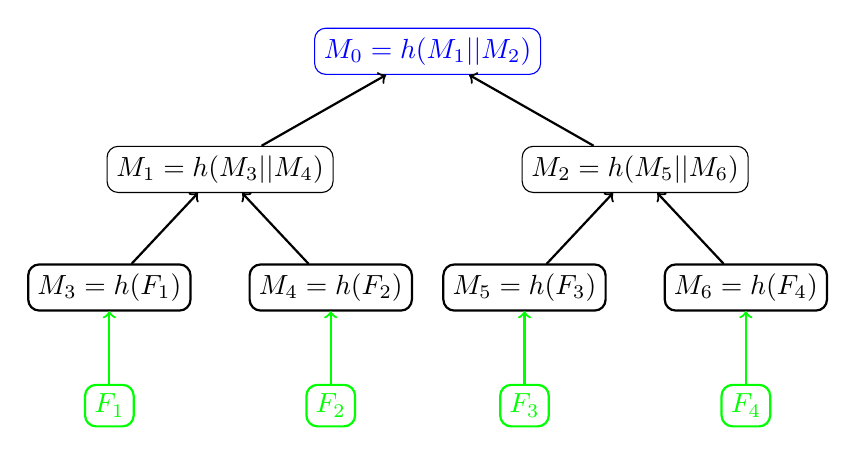
\begin{tikzpicture}[
	sibling distance=15em,
	every node/.style = {shape=rectangle, rounded corners,
	draw, align=center,
	top color=white, bottom color=white},
	level 2/.style={sibling distance=8em},
	level 3/.style={color=green},
	edge from parent/.style={<-,draw,thick}
]
\node[color=blue]{$M_0 = h(M_1 || M_2)$}
	child { node {$M_1 = h(M_3 || M_4)$}
		child { node {$M_3 = h(F_1)$}
			child { node {$F_1$} } }
		child { node {$M_4 = h(F_2)$}
			child { node {$F_2$} } }
	}
	child { node {$M_2 = h(M_5 || M_6)$}
		child { node {$M_5 = h(F_3)$}
			child { node {$F_3$} } }
		child { node {$M_6 = h(F_4)$}
			child { node {$F_4$} } }
	};
\end{tikzpicture}
\caption[A Merkle Tree]{ A graphical representation of a Merkle tree built from a file $F$ split into 4 chunks $[F_1, F_2, F_3, F_4]$.
Here $||$ represents concatenation.}
\label{Merkle example}
\end{figure}

The file chunks are not considered to be part of the Merkle tree when calculating depth, as such the tree in Figure~\ref{Merkle example} has depth 2.



\subsection{Merkle tree Public Proofs of Retrievability}

Merkle trees provide a way to prove membership of a single chunk of a file in $O(\log(n))$ time and space,
whilst requiring the verifier to have only $O(1)$ information (the root hash).

A proof consists of a chunk of the file, and all the other hashes needed to reach the root hash.

Consider Figure~\ref{Merkle example}.
To produce a proof of membership of chunk $F_3$, for example, we include $F_3$ in full.
We do not need to include $M_5 = h(F_3)$, since this can be calculated from $F_3$.
The aim is to compute the root hash, so we include $M_6$ and $M_1$.\\
A verifier then computes the hash of $M_5 = h(F_3)$, followed by $M_2 = h(M_5 || M_6)$
and finally $M_0 = h(M_1 || M_2)$. They then compare $M_0$ to the known root hash.

\begin{figure}[h]
\centering
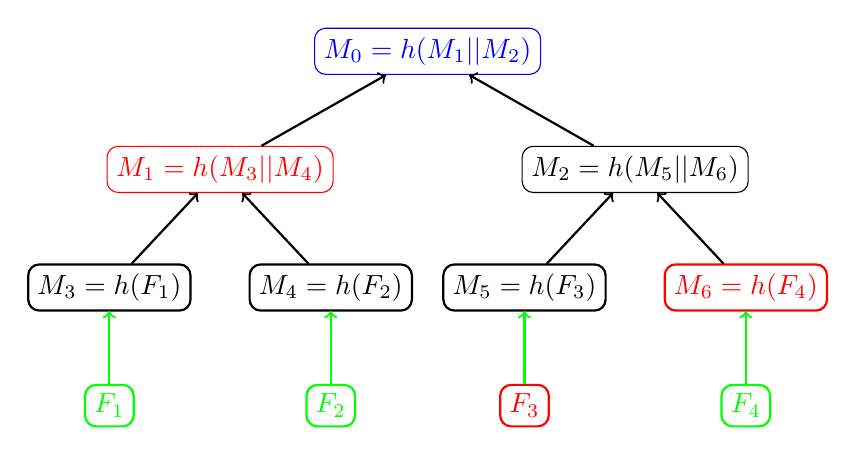
\begin{tikzpicture}[
	sibling distance=15em,
	every node/.style = {shape=rectangle, rounded corners,
	draw, align=center,
	top color=white, bottom color=white},
	level 2/.style={sibling distance=8em},
	level 3/.style={color=green},
	edge from parent/.style={<-,draw,thick}
]
\node[color=blue]{$M_0 = h(M_1 || M_2)$}
	child { node[color=red] {$M_1 = h(M_3 || M_4)$}
		child { node {$M_3 = h(F_1)$}
			child { node {$F_1$} } }
		child { node {$M_4 = h(F_2)$}
			child { node {$F_2$} } }
	}
	child { node {$M_2 = h(M_5 || M_6)$}
		child { node {$M_5 = h(F_3)$}
			child { node[color=red] {$F_3$} } }
		child { node[color=red] {$M_6 = h(F_4)$}
			child { node {$F_4$} } }
	};
\end{tikzpicture}

\caption[A Merkle Tree proof of membership]{A graphical representation of a Merkle tree built from a file $F$ split into 4 chunks $[F_1, F_2, F_3, F_4]$.
Here $||$ represents concatenation.}

\label{Merkle proof}
\end{figure}


Provided the hash function used satisfies the properties in section~\ref{crypto-hash}
for a cryptographic hash, it is not computationally feasible to fake the proof just from the root hash: the file chunk and the relevant hashes (or the file to reconstruct them) are required.

We can use this proof of membership to create a PPoR by making the chunk required dependent on $\kappa$, that is, define
\begin{itemize}
\item $\texttt{extract}(F) = \texttt{root\_hash}(\texttt{Merkle}(F))$


\item $\texttt{generate\_proof}(F, \kappa) =
F_{\kappa \mod m} || \text{Merkle tree hashes forming proof}$

Here $m$ is the number of chunks in the file, with $F_i$ being the $i$th chunk of $F$.

\item $\texttt{verify}(\nu, \kappa, r) =
\texttt{extract\_root\_hash}(r) == \nu$
\end{itemize}



This scheme gives a constant size to $\nu$ and a logarithmic size for the proof $r$.

This scheme certainly isn't a perfect PPoR, for example an adversary storing only half the file and one hash value has a 50\% chance of being able to generate a valid proof.
However to successfully generate a proof the chunk $i \equiv \kappa \mod m$ must be stored.
This means that the chance that an attacker can generate a proof is at most equal to the fraction of the file stored.
This is important because it means it is always more profitable to store the entire file rather than some subset of it, in terms of expected payout per unit storage.

%Formally:
%
%Consider a large file $F$ as a set of equally sized chunks $\{f_1, ..., f_n\}$.
%It is the case that
%for all subsets $F'$ of $F$
%there is no polynomial time function $\texttt{cheat}(c(F), \kappa)$ such that for sufficiently large $F$
%\[\mathbb{P}(\texttt{verify}(\nu, \kappa, \texttt{cheat}(c(F), \kappa)) = 1) > \frac{|F'|}{|F|}\]
%where $c(F)$ is at most $|F'| + O(\log(|F|))$ in size.\\
%That is, the chance of success cannot be greater than the portion of the file that is stored.
%
%This means that it is not more profitable to only store part of a file, provided there is a payout for a valid proof and no consequence for failure.


%\subsection{RSA Homomorphic encryption proof of retrievability}

%





\section{Prior work}

% Currently existing things in the space of using Cryptocurrencies to fuel DFS.
% I also used dieas from several PoR papers which will be discussed when I look at extensions

\subsection{Inspiration for proposal}

I first saw the idea for using Ethereum contracts to fund off chain file storage in the Ethereum Whitepaper \cite{eth-whitepaper}.
In this report I implement and expand on this idea, looking at different implementations and any limitations of Ethereum encountered.
It also suggests a way to recover the files afterwards, though that is not considered here.

\subsection{Proofs of retrievability}

\subsection{Filecoin}

Filecoin is a proposal for a Bitcoin-like cryptocurrency and distributed file system in one
that has a proof of retrievability component along with its proof of work function for block mining.
It's whitepaper \cite{filecoin} points to work on compact public proofs of retrievability by Shacham and Waters \cite{compact-por},
however as far as I know Filecoin has never been implemented.

\subsection{Swarm, SWEAR and SWINDLE}

Swarm is an overlay for a distributed file system (e.g. IPFS \cite{ipfs}), based on Ethereum.
At the time of writing Swarm is currently in alpha on the Ethereum public test chain \cite{swarm-alpha}.

Swarm has two parts, payment channels to incentivise file exchange and a system similar to the one designed here for incentivising long term storage.

I will describe briefly the long term storage incentive proposed in \cite{swarm-swear-swindle}.

If an owner wishes to pay a node in the Swarm network to ensure that a chunk (Swarm is built around fixed size chunks rather than files)
is stored then the owner pay (via a contract) a node and receives a receipt in return and the storer provides a deposit for the contract.
This receipt contains the hash of the chunk and a validity time and is signed by the storing node.

If the owner (or anyone else who has the receipt) believes that their chunk has not been stored then they go back to the contract with the receipt and a deposit.
This is then a challenge, the deposit must cover the cost of uploading the chunk and the receipt must be valid (checked by the contract).
The storer then has some amount of time to upload the entire chunk to the contract, which can then check that the hash matches that of the receipt.

\begin{itemize}
\item If the challenge is successful (there is no valid chunk uploaded) then the challenger is compensated.
\item Otherwise the storer may recover his funds along with the challenger's deposit that covers the chunk upload cost.
\end{itemize}

If a challenge is not received before the receipt becomes invalid the storer may recover their funds.\\

The approach I will take as some benefits over the one given here under the assumptions I operate under.
%Should consider under challenge is always made for one chunk
\begin{itemize}
\item No interaction is required. The owner does not have to make the challenge themselves. Moreover an incorrect challenge will cost the owner in the Swarm scheme.
\item Merkle tree proofs of retrievability are likely to be shorter, and require less information be held by the client, at least for large files.

Consider the implementation used by Swarm, with a chunk size $C$ (4096 bytes in Swarm), and say the owner wants to ensure an entire file $F$ of size $|F|$.
There will be $\frac{|F|}{C}$ chunks and the owner must therefore store $\frac{|F|}{C}$ receipts.
The chunk hash and signature will both be 32 bytes in size (the hashing functions and Elliptic curve cryptography verification function available to the EVM uses 256 bit keys).
The owner must store at least $64 \cdot \frac{|F|}{C}$ bytes. The proof for any given chunk is $C$ bytes, we assume the owner requests a proof for one random chunk.

In comparison, in a Merkle tree scheme the owner stores nothing and the proof size is $C + 32 \cdot \log_2(\frac{|F|}{C})$.
This encourages a chunk size of around 64 bytes. For a 1MB file the proof size is then 512 bytes.
Choosing to make the proof size equal in the Swarm scheme (so $C = 512$ bytes) we find the owner must store $64 \cdot \frac{1 \text{MB}}{512 \text{bytes}} = 131072$ bytes,
or about 13\% of the original file size. This can be reduced by increasing the chunk size, in exchange for higher transaction fees when a challenge is made.
\end{itemize}

The scheme used by Swarm does have a potentially significant advantage that transaction costs are very low if a challenge is never made.
This makes sense for Swarm as we expect the owner to try and recover the files from the Swarm network before resorting to a challenge as insurance.
As such the higher transaction fees are not a significant issue, though if this litigation procedure becomes common Swarm could benefit from building a 64 byte based Merkle tree
from each chunk when considering receipts and litigation as this would decrease the proof size to 256 bytes.

The scheme used by Swarm is simpler, just a single hash operation.
While this is a good thing, to the EVM the extra complexity is cheaper than the larger transaction size.

\section{Solidity}

Solidity is a high-level language that compiles to EVM bytecode.
Originally proposed on August 29th 2014, Solidity is a statically typed object oriented language with JavaScript-like syntax \cite{solidity-proposal}.
It is designed for contract creation and contains several abstractions over EVM code, like dynamically sized arrays, strings and datatypes with sizes smaller than the 256-bit word size.

The language is still in development and their are some limitations not present in EVM bytecode, like the lack of nested dynamic arrays and array slicing \cite{solidity-docs}.

As part of my preparation I learnt to use Solidity and have since used it to write the contract.
The full contract code is included in Appendix \ref{app-contract} if you wish to see an example of Solidity code.


%\section{Requirements analysis}

% Java, Eclipse, geth, Remix, test-chain

%\section{Tools and libraries}


\section{Design of system}

This subsection is a written up version of the plan I made towards the end of the preparation stage to allow me to begin implementing the system.

The system splits into two main components, the proof generator, which I've written in Java, and the contract itself, written in Solidity.
The plan details the structure of the proof and the contract to provide an interface between the two
main components so I could begin writing the Java code whilst still learning Solidity.

There were a couple of minor changes from this plan which are discussed in the Implementation chapter, section \ref{impl-changes}.

%\subsection{Explanation of design}
%
%The solution therefore must require that a proof of retrievability require the file to construct, but can be verified without access to the file.
%It is not necessary that all the file be used in the construction, but it is required that the parts of the file needed cannot be predetermined.
%
%The Merkle tree POR satisfies this.
%
%Merkle tree proofs are only for a single chunk in the file.
%It must not be possible to preemptively guess the index of this chunk or the proof could be precalculated and the file discarded.
%We use the hash of the block before that the contract becomes active (begins accepting proofs).


\subsection{Building the Merkle tree}

To build the Merkle tree I split the file $F$ into $m$ chunks of size $C$, zero padding the final chunk if necessary.
I then append all-zero chunks to the file until the total number of chunks, $M$, is a power of two.
The Merkle tree is then built over this extended chunk set and will have depth $\log_2(M)$.
I denote the root hash of the Merkle tree as $R$.


\subsection{Details of the proof algorithm.}
\label{proof-details}

The proof key is calculated as $\kappa = \texttt{blockhash}(T_0 + N)$
and the index of the file chunk the proof is for is $i \equiv \kappa \mod m$.
This means that the extra all zero chunks will never be selected for proof.

The proof itself is a sequence of bytes containing the selected file chunk $F_i$ and the other hashes from the Merkle tree required to recover the root hash, e.g


\begin{figure}[h]
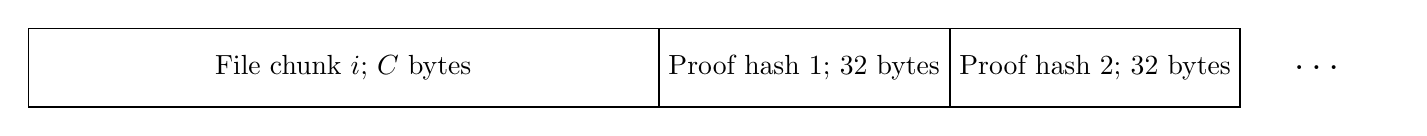
\begin{tikzpicture}

\node[draw,minimum width=8cm,minimum height=1cm](chunk) {File chunk $i$; $C$ bytes};
\node[right=0cm of chunk,draw,minimum width=3cm,minimum height=1cm](hash1) {Proof hash 1; 32 bytes};
\node[right=0cm of hash1,draw,minimum width=3cm,minimum height=1cm](hash2) {Proof hash 2; 32 bytes};
\node[right=0cm of hash2,minimum width=2cm,minimum height=1cm](hash2) {\Large\ldots};

\end{tikzpicture}
\caption[Proof structure]{A representation of the structure of my Merkle tree based PoR proof.}
\end{figure}


To verify the proof, one first hashes the first $c$ bytes, then concatenates it with the next hash in the proof,
hashes this new value and repeats until the end of the proof.
A valid proof is one that results in the root hash being the final value.
The order in which the hashes are concatenated ($A \,||\, B$ or $B \, || \, A$) depends on $i$, as we mirror a walk up the Merkle tree.
Equivalently it can be thought of depending on the binary representation of $i$, from least to most significant bit.

The length of the proof will be $C + 32 \log_2(M)$ bytes, dependant on the size of the file, but not on the selected chunk $i$.
The 32 comes from the 256 bit hash function, SHA-256 used.

%Pseudo-code for the proof generation and verification is reproduced below.
%
%Have function \texttt{readChunk} that reads the next chunk from the file (and implicitly keeps its position).
%\texttt{h} is the hash function, \texttt{||} denotes concatenation and \texttt{array[i, j]} denotes array slicing.
%
%The Java code for these functions may be found in Appendix **.
%The Solidity contract which implements the verification algorithm is in Appendix \ref{app-contract}.


%Should give full example


\subsection{Details of the contract}
\label{contract-plan}

The contract is uploaded to the blockchain at block number $T_0$, containing $X$ ether.
After $N$ blocks it becomes available for submission of proofs.
If a proof is successfully verified the contract pays the sender its $X$ ether and self destructs.

I use the following symbols for variables in the contract:

\begin{itemize}
\item $F$ is the file the contract is for.
\item $m$ is the number of chunks in $F$.
\item $R$ is the root hash of the Merkle tree of $F$.
\item $T_0$ is the block the contract is created on.
\item $N$ is the number of blocks the contract waits before becoming active.
\item $X$ is the amount of ether the contract holds initially.
\item $\kappa$ is the block hash of block $T_0 + N$.
\item $i$ is the chunk of the file a proof for is required, I take $i \equiv \kappa \mod m$.
\end{itemize}

The contract should reject a proof submission if:

\begin{itemize}
\item The contract has already paid out.

%In the implementation the contract destroys itself upon a successful proof validation,
%giving all contained funds to the submitting actor.
%In addition to solving this problem, it means the contract need no longer be stored by nodes,
%so it's creation transaction can be dropped from the blockchain, which is considered good practice.

\item The block number is $\leq T_0 + N$.
\item The block number is $> T_0 + N + 256$ (can't get block hash).

The current block number is available to the contract so these are simple comparisons.

\item The proof is invalid.

\end{itemize}



\section{Review of the preparation stage}

I achieved all of my goals for the Preparation stage of the project.
I built the contract and the proof generation components separately and had them successfully work together with only very minor changes.
%Got a text file with notes specifying the behaviour of the contract and specification of proof format and algorithms


\chapter{Implementation}

\section{Project structure}


There are three black boxes that need to be implemented.
\begin{itemize}
\item Extract -- Find the Merkle tree root hash ($\nu$) from $F$. This is uploaded to the blockchain as part of the contract.
\item Generate proof -- Given a file $F$ and a key $\kappa$ create a proof of retrievability.
\item Verify proof -- Given a root hash $\nu$, a proof $r$ and key $\kappa$ determine whether the proof is valid.
\end{itemize}

I will code the first two in Java.
The algorithms for finding a Merkle tree root hash and for a proof of membership are similar
and in my implementation a lot of the code is reused, so I've treated these as one component for implementation purposes.

The verification is part of the contract, written in Solidity.

\begin{figure}[H]
\centering
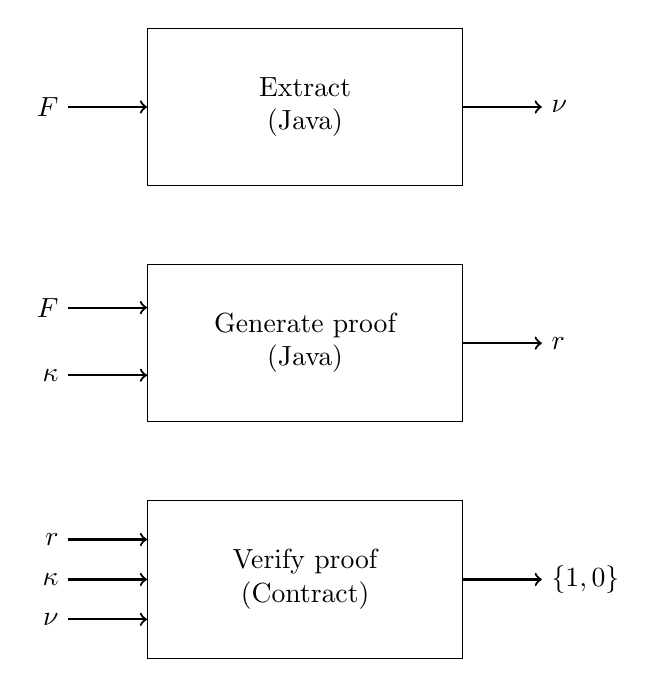
\begin{tikzpicture}
\coordinate(O1) at (0,0);

\node[below=0cm of O1, draw, minimum width=4cm, minimum height=2cm, align=center](a) {Extract\\(Java)};
\node[left=1cm of a](aF) {$F$};
\node[right=1cm of a](anu) {$\nu$};

\node[below=3cm of O1, draw, minimum width=4cm, minimum height=2cm, align=center](b) {Generate proof\\(Java)};
\node[above left=-0.8cm and 1cm of b](bF) {$F$};
\node[below left=-0.8cm and 1cm of b](bi) {$\kappa$};
\node[right=1cm of b](br) {$r$};
\node[right=1cm of bF](bFb) {};
\node[right=1cm of bi](bib) {};

\node[below=6cm of O1, draw, minimum width=4cm, minimum height=2cm, align=center](c) {Verify proof\\(Contract)};
\node[above left=-0.7cm and 1cm of c](cr) {$r$};
\node[left=1cm of c](ci) {$\kappa$};
\node[below left=-0.7cm and 1cm of c](cnu) {$\nu$};
\node[right=1cm of c](cbool) {$\{1, 0\}$};
\node[right=1cm of cr](crc) {};
\node[right=1cm of cnu](cnuc) {};


\draw[->, thick] (aF) -- (a);
\draw[->, thick] (a) -- (anu);
\draw[->, thick] (bF) -- (bFb);
\draw[->, thick] (bi) -- (bib);
\draw[->, thick] (b) -- (br);
\draw[->, thick] (cr) -- (crc);
\draw[->, thick] (ci) -- (c);
\draw[->, thick] (cnu) -- (cnuc);
\draw[->, thick] (c) -- (cbool);
\end{tikzpicture}
\caption[Project structure]{The three functions that need to be implemented.}
\label{project-structure}
\end{figure}


%First the Java code
%\begin{itemize}
%\item \textbf{Merkle tree}
%
%The Merkle tree code is used twice, once to generate the root hash that is placed in the contract and once to generate a proof for a given file chunk.
%
%\item \textbf{
%
%\end{itemize}

% This project splits conceptually into two parts that are connected only by the proof of retrievability
% These are the contract and the proof generator.
% This is mudied somewhat as there is code to generate a contract for a given file by filling in constants such as file size and Merkle tree root hash.

% Basic picture

%Generate MT root, put in contract, put contract on blockchain, generate proof

%The approximate behavior is

%\section{Contract interface}

% One function, submit proof, takes a proof as an array...
% Picture of proof structure

\section{Alterations from proposal}
\label{impl-changes}

There were some minor changes to the original design as the project progressed.

\subsection{SHA256 $\to$ SHA3 KECCAK}

I'm using a different hash algorithm to SHA256, which I mentioned in the proposal.
This is due to me misunderstanding the documentation when I read it at the time.
Whilst SHA256 is available in EVM code it is in the form of a precompiled contract, not a true opcode,
the intention being to prevent the wasting of opcodes in the language.

As I'll mention later array slicing is not yet implemented in Solidity, so at points I
used an assembly language to improve efficiency.
The SHA256 contract isn't as easily available, so instead I switched to KECCAK-256

SHA3's KECCAK-256 function is available as a true opcode in the EVM.
The output is the same size so it's a drop in replacement in the contract, the only downside is having to bring in an external library
to handle it in Java, whilst SHA256 was available from the standard library.

\subsection{Block hash}

This is an implementation detail. The proposal mentoined the use of the block hash of block number $T_0 + N$ as the key value for proof generation and verification.
The block hash of the current block is not available (to code executing in that block), so the contract actually used the block hash of block $T_0 + N - 1$ instead.


\section{Software engineering practices}

%Unit tests!

%Kept testing cycle short, built a CLI for the proof generator and made a script to generate and deploy contracts.

\section{Java proof generator}

% The following main components

%Detailed class structure, cli, what libraries
%Maybe a UML diagram...

The Java code for the base project was fairly straightforward to write as I am familiar with Java.
The code to generate the Merkle tree root hash and proof was written first and the contract generator was written later when I was starting to test the contract and write extensions.

\subsection{Class structure}
\subsubsection{ChunkStream}

This class is a wrapper around a Java file stream that abstracts it into a stream of fixed size chunks.
This component can the be easily tested and it keeps IO code out of the rest of the codebase.

\subsubsection{Merkle}
\label{pseudo-code}
This class is the core of the base project, it wraps around a ChunkStream and has methods for finding the root hash of a file and generating the proofs described in section \ref{proof-details}.

I first implemented this class by building the whole Merkle tree in memory upon initialisation,
 however this can use large amounts of RAM, since the size of the tree grows linearly with the size of the file.
Instead I have rewritten this part of the code so that the root hash and proof construction is done using a recursive function using only $O(\log(|F|))$ space.



I feel this part of the code is sufficiently important to include pseudo-code for in the dissertation.
Here the hash function is \texttt{h} and \texttt{||} denotes concatenation.
I assume there is a function \texttt{readChunk()} that returns the next chunk in the file.

\lstset{
breaklines=true,
basicstyle=\ttfamily\small,
tabsize=4
}
\begin{lstlisting}
fun root_hash(depth) {
    if (depth == 0) {
        return h(readChunk());
    } else {
        return h(merkle(depth - 1) || merkle(depth - 1));
    }
}
\end{lstlisting}

The proof generation for the \texttt{i}th chunk of the file can then also be expressed as a similar recursive function.

\begin{lstlisting}
fun proof(depth, i)
    if (depth == 0) {
        readChunk();
    } else {
        M = 2^(depth - 1);
        if (i < M) {
            return proof(depth - 1, i) || merkler(depth - 1);
        } else {
            tmp = merkle(depth - 1);
            return proof(depth - 1, i - M) || tmp;
        }
    }
}
\end{lstlisting}

For testing reasons I also implemented the validation procedure in Java as well as in the contract.

\begin{lstlisting}
fun validate(chunkSize, rootHash, proof, i) {
    
    depth = (proof.length - chunkSize) / hashLength;
    hash = h(proof[0, chunkSize]);
    int positionInProof = chunkSize;
    
    for n in 0..(depth-1) {
        otherHash = proof[positionInProof, positionInProof + hashLength];
        if (i % 2 == 0)
            hash = h(hash || otherHash);
        } else {
            hash = h(otherHash || hash);
        }
        i /= 2;
        positionInProof += hashLength;
    }
    return hash == rootHash;
}
\end{lstlisting}

The full Java code for these three functions can be found in Appendix~\ref{app-java}.

\subsubsection{ContractGenerator}

Whilst I was developing the contract I found that the process for deploying the contract to a local blockchain was very cumbersome, so
I added additional code to the Java part of the project to generate contracts by filling in file specific constants like the number of chunks and the Merkle tree root hash.
The contract is then packed into a JavaScript file for the \texttt{geth} Ethereum client to run, which deploys the contract ready for testing.
This made it much quicker to test the behaviour of the contract on different files as well as making it possible to write some semi-automated tests by altering the deployment script.

\subsection{Command line interface}

I added a simple command line interface to the program as I built it allowing me to easily test the code with different files and chunk sizes,
as well as later being able to run the extensions as optional flags for the program.
For this I used the Apache Commons CLI library.

\subsection{Testing}

I wrote several unit tests for the ChunkStream class, particually checking behaviour in edge cases like the last block of a file, which should be padded with zeroes.

I also wrote unit tests for the Merkle class to make sure the proof was correct since it is the interface with the contract.

I used the JUnit 4 testing framework.

\subsection{Tools}

I used Java 7 with the Eclipse IDE for this part of the project.
I used the following libraries.
\begin{itemize}
\item Apache Commons CLI (Apache license)
\item RNRT SAPHIR, for the KECCAK-256 hash function (MIT-like and BSD-like licenses)
\item JUnit for unit tests (Eclipse Public License)
\end{itemize}
%Eclipse, commons CLI


\section{Contract}

I wrote the contract in Solidity.
Although there is less code than the Java part the contract took longer to write due to my unfamiliarity with the language and
some issues which had to be resolved along the way.

\subsection{Structure}

For ease of writing and reading the contract is split into two main functions, though they are just called sequentially when
the main entry point \texttt{submitProof} is run.
There are also a few small functions that provide information about the contract's state for testing, as well as a simple
constructor (which is run when the contract is deployed) which records the initial block number $T_0$ and address of the contract's owner.

\subsubsection{validToCall}

This function performs the checks listed in the design plan of section \ref{contract-plan}.
\begin{itemize}
\item The block number is $> T_0 + N$.
\item The block number is $\leq T_0 + N + 256$.
\end{itemize}

\subsubsection{validateProof}

This function validates the Merkle tree proof of retrievability against the stored root hash using the \texttt{validate} algorithm in section \ref{pseudo-code}.
The proof is received as a fixed-size array, so the contract must be altered for different files.
Fixed size arrays are more performant, easier to use in the inline assembly and preclude a series of potential bugs with trying to submit different size proofs than
should be used for the file.


%\subsection{Difficulties}

\subsection{Tools}

I used the online IDE Remix \cite{browser-solidity} for development, and tested it on a private chain using the go-ethereum client \texttt{geth}
solidity compiler \texttt{solc}.
The contract is all my own code and has no dependencies.

% Used solidity, no external dependancies, several functions that are helpful with testing and debugging.


\section{Difficulties with the contract implementation}

I encountered several problems during implementation of the base contract, however I was able to work around them all with no major issues.
I detail a few of these problems here.

Ethereum itself is in `beta', expecting breaking changes, and its ecosystem is young and still developing.
I knew this before proposing the project and planed in extra time to deal with any problems implementing and testing the contract.

\subsection{Documentation}

Though there is central documentation for Solidity which has been very helpful, it is brief and incomplete in places and this slowed down my development of the contract.
For example there is little detail on lesser used keywords (like \texttt{internal}, \texttt{constant} and \texttt{modifier}), especially when compared to the usually very thorough documentation for the Java standard library.

\subsection{Array slicing}

The contract receives proofs as arrays and has to hash slices (subsections) of those arrays.

Solidity does not support array slicing (that is, taking part of an array by using a pointer to the same memory rather than making a copy).
I wanted to avoid making a copy for performance reasons.


%Anecdotally, this is also the case in Java, though it can be worked around with wrapper objects like \texttt{ByteBuffer}.

%\subsection{Libraries}
%
%% not reall improtant?
%Solidity does not come with a standard library. The only extra functions available are those implemented as EVM opcodes or precompiled contracts.
%There is no central place for Solidity libraries (*** was created while my projects was in development).

\subsection{Tooling}

There is an online IDE for Solidity\cite{browser-solidity} which is suggested by the documentation.
This generally worked well, however code execution is very slow and it would sometimes hang or run out of memory.
Being JavaScript based it cannot deal with the EVM's 256-bit word size natively, so large arguments have to be input as zero-padded hex strings.

As far as I can tell the files generated by the offline compiler \texttt{solc} cannot be interpreted by \texttt{geth}, the Ethereum command line client.
A workaround is to call the Solidity compiler from within \texttt{geth}'s JavaScript console,
however JavaScript doesn't support multi-line strings.
For this reason my Java contract generator removes newlines from contracts and creates a script to deploy them from \texttt{geth}.

This has mostly worked well as Solidity does not assign a particular meaning to newlines, except in the case of line comments (\texttt{//}) and inline assembly,
which does not use semicolons to separate expressions.



%%later
%\subsection{Limitations of the EVM}
%
%% No ECC primitives
%
%% No modexp precompile
%
%\subsection{Java and Solidity}
%
%There were a few hard to find bugs in the project that resulted from interoperating between Java and Solidity.
%
%Java's \texttt{BigInteger}, which I make extensive use of in the RSA extension gives a two's complement representation
%when asked for a \texttt{byte[]} representation, which was not useful to me as I was dealing with modular arithmetic and did not need negative numbers.
%This means in particular that, for example, a 256 bit number may take 33 bytes to represent, and attempting to store it in a 32 byte array
%will not produce the desired result in some cases.
%It also becomes an issue when trying to hash \texttt{BigInteger}s in a way that is consistent with Solidity.
%Java \texttt{BigInteger}s have to be converted to byte arrays and then padded or shortened before hashing and reconstructing a \texttt{BigInteger}
%using the hash result as magnitude to produce the desired result.
%To convert to a format that is understood by the JavaScript interface it is necessary to convert it to hex and left pad the result with zeroes
%(and put it in a string starting with \texttt{0x}), because values are otherwise implicitly right-padded to 32 bytes by default.

\section{Security considerations}

There are several edge cases and other implementation details I had to consider to ensure the contract behaves correctly.
The correctness of the proof algorithm has already been considered.
I assumethat the Ethereum network and our hashing algorithm are not compromised.

\subsection{Block hash as random number}

I use the block hash of some block that has not yet been created when the contract is deployed the key $\kappa$.
Anyone wishing to control the block hash would have to generate blocks ahead of the main network
and discard them until they found one they wanted.
Discarding blocks increases the risk that another node will create the block first meaning loss of the block reward, which is likely to
far exceed anything gained from manipulating a contract of this kind (at the time of writing the block reward is 5 Ether or about 250 USD).

\subsection{File length is not a multiple of chunk size}
\label{file-len-chunk-size}

In this case there is less information contained in the final chunk of the file, as it is zero padded in my implementation.
This means storing the last block of the file is more profitable (per byte stored), as it uses less space.

One way to solve this would be to pad files with random bits to a multiple of the chunk size before using the contract.
%This problem is partially solved by requiring a storing node to pay a deposit as a promise they will keep the file.

\subsection{Number of chunks, $m$, is not a power of two}
\label{file-len-chunk-num}

The number of leaf nodes in the Merkle tree (in my implementation) must always be a power of two.
The extra blocks are treated as all zero when building the tree, though they will never be selected for proofs.
This was done for simplicity of implementation.

This means that if you are only storing a subset of the chunks, plus extra hashes to allow proof construction,
then some will require slightly less extra data.
However it is still more profitable per chunk stored to keep the whole file and be able to reconstruct the Merkle tree as required.

%If the actor stores the whole file then the payout per chunk is $\frac{X}{m}$.
%If the actor were to only store $n < m$ chunks then they must store a strictly positive amount of extra data, $\epsilon$, to be able to reliably construct a valid proof for those $n$ chunks.
%The chance that one of these $n$ chunks is chosen is $\frac{n}{m}$.
%Therefore the expected payout per chunk is $\frac{n}{m} \cdot \frac{X}{n + \epsilon} = \frac{X}{m + \epsilon'} < \frac{X}{m}$
%and the actor will always store the whole file.
%
%This breaks down if the actor cannot store the whole file in which case it can cause some sets of chunks to be more valuble than others.
This edge case is a good reason to implement the lock-in extension (see section \ref{ext-lockin}).

\subsection{Block hash availability}

The last 256 block hashes are available to code executing in the EVM, not including that of the current block.
The EVM opcode that retrieves a block hash fails silently if that block is not available, returning 0.
As such the block hash used as the key $\kappa$ must be before the contract becomes active,
and the contract must deactivate 256 blocks later, rejecting further proof submissions.

There are methods to get round this limit on block has availability, however with a block time averaging 14 seconds
256 blocks is about one hour, which is plenty of time to create a proof and submit the transaction.

\subsection{Multiple rewards}

If the contents of the file is very important to the owner then they may want multiple nodes in the network to keep copies of the data.
Simply allowing the contract to pay out to multiple Ethereum addresses will not work as one node could store the file once and claim all the rewards
using different addresses.
A better way for the owner to increase their confidence in the files security would be two encrypt the file with different keys and
upload multiple versions of the file with separate contracts.

\section{Configuration}

\subsection{Effect of chunk size}

\subsubsection{Performance of proof generation}

In general, larger chunk sizes improve performance simply because the Merkle tree will have fewer nodes and so take less time to build.

\subsubsection{Proof size} \label{chunk-size-proof-size}

Recall that the proof is the chunk concatenated with all the hashes required for a Merkle tree proof of membership.

Let the chunk size be $c$ bytes.
The number of chunks for a file $F$ is therefore $\frac{|F|}{c}$.
The depth of the Merkle tree is $\left\lceil\log_2\left(\frac{|F|}{c}\right)\right\rceil$.

We use a hash algorithm with 256-bit (32 byte) output, so the proof size is
\[|r| = c + 32 \cdot \left\lceil\log_2\left(\frac{|F|}{c}\right)\right\rceil\]

\begin{figure}[h]
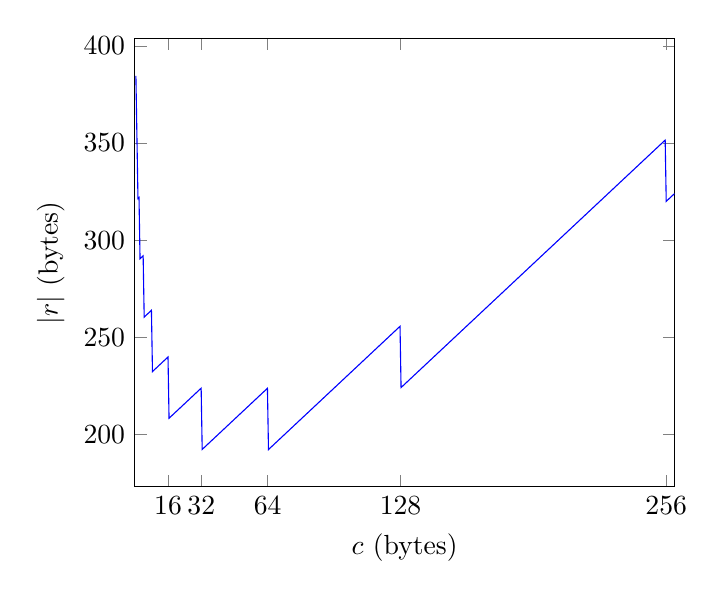
\begin{tikzpicture}
  \begin{axis}[ 
    xmin=0, xmax=260,
    xlabel={$c$ (bytes)},
    ylabel={$|r|$ (bytes)},
    domain=0:260,
    samples=522,
    xtick={16, 32, 64, 128, 256},
  ]
    \addplot[color=blue,mark={}]{x + 32 * ceil(log2(1024 / x))}; 
  \end{axis}
\end{tikzpicture}
\caption[Chunk size graph]{Proof size against chunk size for a 1024 byte file.}
\label{eval-graph-chunk-size}
\end{figure}


The size of the proof will always be smallest when $F/c$ is a power of two due to the Merkle tree always being a power of 2 in size.

We wish to find the chunk size that will minimise the size of the proof.
If we require $|F|$ to be a power of two then this analysis is simple.
Since $F/c$ is a power of 2 at the minima, it follows $c$ is a power of two in this case and we find
\[|r| = c + 32\log(c) + 32\log_2(|F|)\]
and so we can simply minimize $c + 32\log(c)$ with respect to $c$, finding that 32 and 64 bytes both give minima.
Since proof generation benefits from larger chunk sizes I choose 64 bytes as the default chunk size.

If we don't require $|F|$ to be a power of two then this doesn't hold, the full analysis is included in Appendix~\ref{app-chunk-size}

\section{Extensions}


\subsection{Recovery}

This is an important extension for practical purposes.
The contract should allow the owner to recover the funds in the contract if no-one submits a valid proof before the 256 block expiration.

To implement this the contract stores the address of its creator as it is created
and allows the owner to recover the funds (and destroy the contract) after block $T_0 + N + 256$.

\subsection{Lock in} \label{ext-lockin}

The contract can be redesigned such that a storage node must lock in a certain amount of funds before some time $T_0 + N'$ (where $N' < N$),
to allow them to claim the reward later.

This would give the owner confidence that their file is stored, and discourage storage nodes from only storing a subset of the chunks in a file,
or deleting stored data if a more lucrative contract becomes available.

The contract is initially loaded with $X$ Ether by the owner.
One storage node can send $L$ Ether to the contract, their address is then stored on the blockchain by the contract.
When a proof is submitted the contract will check that the address matches, and return $X + L$ Ether to the node
on submission of a valid proof.

If the node does not submit a valid proof while the contract is active, then the full $X + L$ Ether can be recovered by the owner.

\subsection{Multiple chunk proofs} \label{multi-chunk}

One way to improve the relationship between expected profit and the fraction of file stored
when using the Merkle tree PPoR is to require proofs of membership for $Y$ chunks in the file.
In this case, for a node storing only $m'$ out of the $m$ chunks in the file, the chance that a proof can be successfully created for $Y$ selected chunks is
approximately equal to $\left(\frac{m'}{m}\right)^Y$,
which discourages storing a small portion of a file.
The main downside is that the size of the proof now grows linearly with $Y$.

Different chunk numbers for proofs are be extracted from the block hash $\kappa$ by hashing is $Y$ times and taking the value modulo $m$
as the chunk index each time.
This means the chunks are selected with replacement.

I have implemented this extension as a command line option for proof generation and as an alternative version of the contract.


% What it could do it theory



%\subsection{Multiple Merkle trees}
%
%It is possible to alter how the file is split up into chunks. So far we have simply divided the file evenly into parts, however there is no reason we couldn't have taken strips of the file instead.
%
%\begin{figure}[h]
%\begin{tikzpicture}
%
%\node[draw, minimum width=2cm,minimum height=3cm,fill=yellow!30](chunk1) {};
%\node[right=0cm of chunk1,draw, minimum width=2cm,minimum height=3cm,fill=red!30](chunk2) {};
%\node[right=0cm of chunk2,draw, minimum width=2cm,minimum height=3cm,fill=blue!30](chunk3) {};
%\node[right=0cm of chunk3,draw, minimum width=2cm,minimum height=3cm,fill=green!30](chunk4) {};
%
%\end{tikzpicture}
%\caption[]{Chunks}
%\label{file-chunk}
%\end{figure}
%
%\begin{figure}[h]
%\begin{tikzpicture}
%
%\node[draw, minimum width=0.5cm,minimum height=3cm,fill=yellow!30](chunk1) {};
%\node[right=0cm of chunk1,draw, minimum width=0.5cm,minimum height=3cm,fill=red!30](chunk2) {};
%\node[right=0cm of chunk2,draw, minimum width=0.5cm,minimum height=3cm,fill=blue!30](chunk3) {};
%\node[right=0cm of chunk3,draw, minimum width=0.5cm,minimum height=3cm,fill=green!30](chunk4) {};
%
%\node[right=0cm of chunk4,draw, minimum width=0.5cm,minimum height=3cm,fill=yellow!30](chunk1) {};
%\node[right=0cm of chunk1,draw, minimum width=0.5cm,minimum height=3cm,fill=red!30](chunk2) {};
%\node[right=0cm of chunk2,draw, minimum width=0.5cm,minimum height=3cm,fill=blue!30](chunk3) {};
%\node[right=0cm of chunk3,draw, minimum width=0.5cm,minimum height=3cm,fill=green!30](chunk4) {};
%
%\node[right=0cm of chunk4,draw, minimum width=0.5cm,minimum height=3cm,fill=yellow!30](chunk1) {};
%\node[right=0cm of chunk1,draw, minimum width=0.5cm,minimum height=3cm,fill=red!30](chunk2) {};
%\node[right=0cm of chunk2,draw, minimum width=0.5cm,minimum height=3cm,fill=blue!30](chunk3) {};
%\node[right=0cm of chunk3,draw, minimum width=0.5cm,minimum height=3cm,fill=green!30](chunk4) {};
%
%\node[right=0cm of chunk4,draw, minimum width=0.5cm,minimum height=3cm,fill=yellow!30](chunk1) {};
%\node[right=0cm of chunk1,draw, minimum width=0.5cm,minimum height=3cm,fill=red!30](chunk2) {};
%\node[right=0cm of chunk2,draw, minimum width=0.5cm,minimum height=3cm,fill=blue!30](chunk3) {};
%\node[right=0cm of chunk3,draw, minimum width=0.5cm,minimum height=3cm,fill=green!30](chunk4) {};
%
%\end{tikzpicture}
%\caption[A blockchain]{chunk striping}
%\label{file-chunk-stripe}
%\end{figure}
%
%In this case a chunk consists of several strips, one from each of what would originally been each chunk.
%
%Each different way of splitting up the file will produce a different Merkle tree.
%Only one would be required for the proof, selected based on $\kappa$.
%This means several root hashes will need to be stored in the contract (so $\nu$ becomes larger),
%however the size of the proof doesn't change.
%
%*** I think this means we get an exponent in the number of different trees, same as last time, provided the striping is `orthogonal' in some sense ***
%
%This approach would make contract generation significantly slower
%and possibly proof generation as well, especially because the chunks cannot be read sequentially
%which would pose problems when considering large files on mechanical drives.
%

\subsection{Erasure codes}

Erasure codes (or Forward Error Correcting codes in Networking) allow a file to be recovered even if part of the data is lost.

%actually do this.


\subsection{ECC}

It is possible to use techniques based on Elliptic Curve Cryptography (ECC) to create compact public proofs of retrievability.
These techniques have significant advantages over the Merkle tree method I have described; they allow the chance
that a node will be able to generate a valid proof without holding the whole file to be made arbitrarily small whilst keeping the proof compact.

I've looked into implementing the scheme described by Juels and Kaliski\cite{ecc-por} as an extension, to replace Merkle tree based proofs.
The operations required are considerably more computationally expensive than Merkle trees.
Whilst in theory it should be possible to implement them in Solidity, it is likely that the resulting code would be too expensive to run in practice.
There is currently a proposal underway to add native code implementations of elliptic curve primitives
as precompiled contracts in the EVM\cite{eip-ecc}, but unfortunately it will not be deployed before my project is finished.

I have not attempted this extension and instead have attempted a similar extension using RSA primitives.


\section{RSA extension}

It is possible to use RSA as a homomorphic encryption scheme to create public proofs of retrievability.
Similarly to the ECC variants these can be more compact than Merkle tree proofs whilst also having better security properties.
This extension was done in lieu of the ECC extension in the proposal.

Ethereum does not have precompiled primitives for RSA operations, which again means a full implementation
would be prohibitively expensive to run on the blockchain.
There is a proposal underway, similar to the ECC one, to add a precompiled contract for modular exponentiation in the next Ethereum hard fork \cite{eip-rsa},
however it will not be deployed in time for me to use.
This makes it impractical to use a large RSA modulus so instead I have implemented a proof of concept using 256-bit RSA, which is no longer considered to be secure[***].
This is possible to implement from scratch with reasonable performance due to the EVM's 256-bit word size.



\subsection{Homomorphic encryption using RSA}

Let $e$, $p$ and $q$ be large primes and $N = p \cdot q$.
Let $d$ such that $e d \equiv 1 \mod (p-1)(q-1)$ (this can be done efficiently with Euclid's extended algorithm).

Now we have $(m^e)^d \equiv m \mod N$ for all $m \in \mathbb{N}_N$  (where $\mathbb{N}_N = \{n \in \mathbb{N} \,|\, n < N\}$).
Given $e$ and $N$ it is hard to find $d$ unless $p$ and $q$ are known as well.
This therefore forms a public key encryption system with public key $(e, N)$ and private key $d$.

Notice that $(m_1^e \cdot m_2^e)^d = \left((m_1 \cdot m_2)^e\right)^d \equiv m_1 \cdot m_2 \mod N$, so we can perform multiplication on
encrypted messages $m^e \mod N$.
Similarly $\left(\left(m^e\right)^x\right)^d = \left(\left(m^x\right)^e\right)^d \equiv m^x \mod N$, so we can perform exponentiation on encrypted messages.
That is to say RSA is homomorphic under multiplication and exponentiation.

\subsection{RSA public proof of retrievability}

I use a modified version of that described by G. Ateniese et al.\cite{rsa-por}.

%File F, m is no. chunks...

\subsubsection{Initialisation}

Generate RSA keys $N$, $e$ and $d$.
Generate random numbers $v$ and $g$.
Publish all of these values except $d$, which is used for tagging and then deleted.

Let $h$ be a cryptographic hash function and define
$W_i = h_v(i)$.

\subsubsection{Tagging chunks}

In this scheme each chunk of the file $F$ has a tag associated with it that is given to the storage node at $T_0$.

Let $T_i = \left(W_i^{-1} \cdot g^{F_i}\right)^d \mod N$.
%We require that all $F_i$ are less than $N$.

\subsubsection{Proof generation}

We are given a new key $\kappa$ (the blockhash), the public key $(N, e, g)$ and a number of chunks to generate proofs for, $c$.

Use $\kappa$ to select a subset of the chunks in $F$, $\{F_{i_1}, F_{i_2}, \ldots, F_{i_c}\}$ to use in the proof.

Let $a_j = h_\kappa(j)$.

Compute $T = T^{a_1}_{i_1} \cdot T^{a_2}_{i_2} \cdot \ldots \cdot T^{a_c}_{i_c} \mod N$.

Compute $U = a_1 \cdot F_{i_1} + a_2 \cdot F_{i_2} + \ldots + a_c \cdot F_{i_c}$.

Output the proof $(T, U)$.

\subsubsection{Proof verification}

Use $\kappa$ to select a subset of the chunks in $F$, $\{F_{i_1}, F_{i_2}, \ldots, F_{i_c}\}$ (in the same way as before) to use in the proof
and let $a_j = h_\kappa(j)$ as before.

Let $\tau = T^e \cdot W_{i_1}^{a_1} \cdot W_{i_2}^{a_2} \cdot \ldots \cdot W_{i_c}^{a_c} \mod N$.

The verification is successful if $g^U \equiv \tau \mod N$.

\subsection{Notes on the algorithm}

I will try and give some insight into why this proof process works.

We can expand the computation of $T$ in the proof generation section using the definition of $T_i$:
\[T = T^{a_1}_{i_1} \cdot T^{a_2}_{i_2} \cdot \ldots \cdot T^{a_c}_{i_c} =
\left(W_{i_1}^{-a_1} \cdot W_{i_2}^{-a_2} \cdot \ldots \cdot W_{i_c}^{-a_c} \cdot g^{a_1 F_{i_1}} \cdot g^{a_2 F_{i_2}} \cdot \ldots \cdot g^{a_c F_{i_c}}\right)^d\]
(I have omitted the mod $N$ for simplicity and will continue to do so).

In the proof verification we then compute $T^e$ which, since $e$ and $d$ are an RSA pair, will be equal to
\[W_{i_1}^{-a_1} \cdot W_{i_2}^{-a_2} \cdot \ldots \cdot W_{i_c}^{-a_c} \cdot g^{a_1 F_{i_1}} \cdot g^{a_2 F_{i_2}} \cdot \ldots \cdot g^{a_c F_{i_c}}\]
Now we can see that
\[\tau = T^e \cdot W_{i_1}^{a_1} \cdot W_{i_2}^{a_2} \cdot \ldots \cdot W_{i_c}^{a_c} = g^{a_1 F_{i_1}} \cdot g^{a_2 F_{i_2}} \cdot \ldots \cdot g^{a_c F_{i_c}}\]
which should be equal to $g^U = g^{a_1 \cdot F_{i_1} + a_2 \cdot F_{i_2} + \ldots + a_c \cdot F_{i_c}}$.

Here $W_{i_1}^{-a_1}$ means the multiplicitive inverse of $W_{i_1}$ modulo $N$ (which can be found with Euclid's extended algorithm)
raised to the power of $a_1$.

In my implementation the keyed hash function $h_k(x)$ is just KECCAK-256$(k || x)$\footnote{The KECCAK family are secure against length-extension attacks, so that is not an issue here.}.


I have made three changes to the algorithm to ease implementation and improve performance for the contract compared to what is described by G. Ateniese et al.

In the paper the chunks selected for proof were chosen via a keyed permutation.
For simplicity I just repeatedly hashed $\kappa$ and used the value modulo $m$, the number of chunks in the file.
This has the disadvantage that chunks can be selected multiple times but does not break the algorithm.

In the paper the RSA key generation is done using safe primes, that is to say that $p = 2p' + 1$ and $q = 2q' + 1$ are selected
such that $p, p', q$ and $q'$ are all prime and the RSA modulus is $N = pq$.
This allows them to select $g$ as a generator of the quadratic residue group modulo $N$, which ensures
that the order of $g$ is large and therefore the discrete logarithm problem is hard for $g$
(given $g$ and $g^U \mod N$ is is hard to find $U$).\\
I've ommited this constraint on key generation in my proof of concept implementation for simplicity.
The discrete logarithm problem is still hard for most values of $g$ (RSA relies on this), but
the constraint should be included if this scheme were to be deployed.

The original paper defined tagged chunks with a positive exponent ($T_i = \left(W_i \cdot g^{F_i}\right)^d \mod N$)
and used a negative exponent in the proof verification step instead.
I have swapped these around to avoid having to run Euclid's algorithm for the multiplicative inverse in the contract.
I believe this has no influence on the security of the scheme.


\subsection{Merits of this approach}

This scheme is considerably more complex than the Merkle tree version, and this is reflected in the higher gas cost of the contract's execution.
It also has the disadvantage of requiring the storing node to keep the tags along with the original file.

As discussed in section \ref{proof-details}, for a file of $m$ chunks of size $C$, the size of a Merkle tree proof is $C + 32 \log_2(M)$, where $M$ is the least power of two greater than or equal to $m$.
For this scheme the size of $T$ will be the same as the RSA modulus, whcih I will denote as $|N|$,
and the size of $U$ will be $C + |a| + c$, where $|a|$ is the length of the constants $a_i$, which is 256 bits in my implementation,
and $c$ is the number of chunks selected to be in the proof.

This means that the size of the proof increases by only 1 bit for each chunk the proof includes,
whereas the Merkle tree version requires a complete proof for each extra chunk.
In fact it is practical to request a proof for the entire file under the RSA scheme.
In this case a storage node can only create a correct proof when storing the entire file.
The proof is also independent of the size of $F$, provided that we fix $c$ and $C$.

The algorithm is more computationally expensive than the Merkle tree version (especially if a larger RSA modulus is used).
One way to improve the run time of the algorithm (which is mentioned in the paper) is to set all $a_i$ to one,
which means that the proof verification procedure only requires two exponentiations along with several multiplications.
In this case we only have a proof that the sum of the chosen blocks and the product of the chosen tags was available to the storage node.
This is an acceptable trade-off provided the number of chunks $m$ is large and $c$ is not either very small or too close to $m$,
since the number of chunk combinations (in the case of a true permutation being used for chunk selection) is $\begin{pmatrix}m\\c\end{pmatrix}$.


\subsection{Implementation}

I have implemented and tested this algorithm, including the proof generation and contract code.
What I present is a proof of concept and should not be considered secure.%, as previously mentioned I use a small 256-bit RSA modulous and I also
%don't use a cryptographically secure random number generator for key generation.

I implemented the key generation, file tagging and proof generation in Java as an extension to the existing code base for the rest of the project.
I used Java's BigInteger class which has methods for the multiplication, modular exponentiation and addition operations that I needed.

I've also implemented the verification algorithm in Solidity.
The behaviour of this contract is identical to the to the Merkle tree version apart from the proof verification function.
Solidity does not have a big integer library or a library for modular exponentiation.
It does have arbitrary precision \texttt{addmod} and \texttt{mulmod} functions (which are EVM opcodes) for 256-bit inputs,
which I made use of instead of implementing big integers myself.
I did implement modular exponentiation for 256-bit words as a Solidity function.
I used EVM assembly for parts of the proof verification function to reduce gas cost
as it was significantly slower than the Merkle tree version.




\subsection{Implementation difficulties.}

\subsubsection{Java and Solidity}

There were a few hard to find bugs in the project that resulted from interoperating between Java and Solidity.

Java's \texttt{BigInteger}, which I make extensive use of in the RSA extension gives a two's complement representation
when asked for a \texttt{byte[]}, which was not useful to me as I was dealing with modular arithmetic and did not need negative numbers.
This means that, for example, a 256 bit number may take 33 bytes to represent and attempting to store it in a 32 byte array
will not produce the desired result in some cases.
It also becomes an issue when trying to hash \texttt{BigInteger}s in a way that is consistent with Solidity.
Java \texttt{BigInteger}s have to be converted to byte arrays and then padded or shortened before being hashed and then resulting byte array
used as a magnitude to reconstruct a \texttt{BigInteger}.
To convert \texttt{BigInteger}s into a format that is understood by the JavaScript interface it is necessary to convert them to hex and then left pad the result with zeroes
(and put them in a string starting with \texttt{0x}), because values are otherwise implicitly right-padded to 32 bytes by default.
I discovered all of these things %by rereading the documentation or by trial and error
after discovering my first implementation did not work.






\chapter{Evaluation}

\section{Overview}

I have successfully implemented the system described in my original proposal with only a few modifications.
In addition I have implemented several extensions, some of which were mentioned in my proposal and some of which
I only thought of as the project progressed.
%What was implemented, which extensions

This chapter will look at the base system and the various extensions in terms of their performance and the expected profit of a
storage node trying to cheat.

\section{Performance}

%Graphs!

\subsection{Time to generate proofs}

The time taken to generate the proof for a file (and to find the root hash for contract generation) should be as low as possible.

It must be possible to generate the proof in the 256 blocks ($\approx 1$ hour)  that the contract is active for,
though in practice this is not an issue, at least for the base contract.

The following graph is for the base contract.
The test was done on my own PC (i3-4330@3.5GHz, 8GB, Samsung 850 Evo SSD).

\subsection{Execution cost of contract}

\subsubsection{Deployment cost}

There is a cost associated with deploying a contract to the blockchain.
The cost is dependent on the code size of the contract.
This cost could be mitigated by creating a reusable contract, or even using one contract to cater for many different files, though I have not implemented this.
The deployment cost of the base contract is *** gas and the various extensions only slightly increase this

\subsubsection{Cost of proof submission}

To be practical to use the transaction cost of submitting a proof must be reasonably low
and must scale well with large files.

Figure ** is a graph of file size, $|F|$, against transaction cost for the submission of a correct proof.
The transaction cost grows logarithmically with the size of the file, which is expected as the size of the proof and complexity of the verification algorithm are both logarithmic in $|F|$.
To give some context, one gas is currently worth *** Ether and one Ether is currently worth £***, meaning a 1kb file would cost about *** in transaction fees and
a 500MB file would cost about ***.

Whilst the cost for large files is reasonable, the transaction cost for small files may be prohibitive...

\subsubsection{Multiple proof chunks}

\subsubsection{RSA extension}


\section{Expected profit of attacker}


\subsection{Model}

I want to evaluate the expected profit of a storage node in terms of how many chunks of a file it stores.
I model the system under the assumption that a storage node gets a fixed reward of $X$ Ether for providing a correct proof and nothing for an invalid proof
or not providing a proof at all.

We make several simplifying assumptions.
\begin{itemize}
\item I ignore the logarithmic amount of extra data required to build a Merkle tree from a file chunk.
This is generally a reasonable assumption, for example an actor storing one half of the file needs only one extra hash stored to
construct valid proofs for the 50\% of chunks they have stored.

\item I also assume it is impossible to create a correct proof without having the relevant chunk of the file,
ignoring the tiny chance that the storage node can guess a correct proof.

\item I assume every chunk is equally sized and equally valuable (see section \ref{file-len-chunk-size} and \ref{file-len-chunk-num}).

\item I ignore transaction fees. One may consider $X$ to be the original Ether placed in the contract minus the transaction fee for verifying a proof.
Since contract execution is deterministic (assuming the block the transaction will be included in is known and no conflicting transactions are processed before hand) it is 
always possible to know whether a proof submission will succeed by running the code offline, so one would expect an invalid proof would never be submitted.
\end{itemize}


Let $F'$ be the set of chunks stored by the actor. I write $\frac{|F'|}{|F|}$ for the fraction of the chunks stored.

I consider two threat models
\begin{itemize}
\item A storage node that wishes to maximise its expected profit per unit storage.

This is a logical actor working in the network and one would hope that the system will encourage them to always store the whole file.

\item A storage node that stores only enough of the file to break even.

This could be a logical node that has limited storage space available, but will store part of a file if it can still make a profit.
Ideally a node should only be able to make a profit if they store enough of the file for the owner to recover it, and this can be accomplished with erasure codes.
\end{itemize}

Malicious nodes, which are willing to work at a loss, are considered to be outside of the threat model for this report.

\subsection{Base implementation}

In the base system, under these simplifications,
the expected profit varies directly with the proportion of chunks stored.
This is because, under these assumptions, a proof can be created if and only if the relevant chunk of the file is stored.
\[E(\text{profit}) = X \cdot \frac{|F'|}{|F|}\]
The expected profit per unit storage is then constant at $\frac{X}{|F|}$.

\begin{figure}[H]
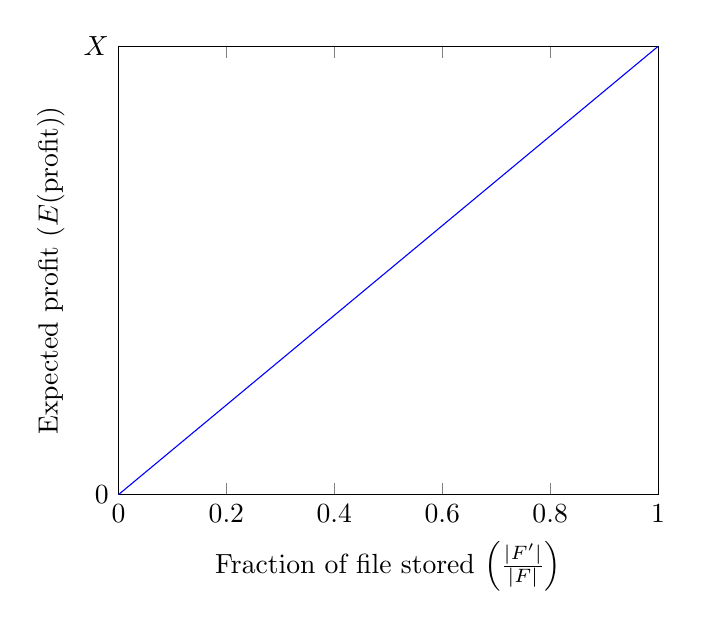
\begin{tikzpicture}
  \begin{axis}[ 
    xmin=0, xmax=1,
    ymin=0, ymax=1,
    xlabel={Fraction of file stored $\left(\frac{|F'|}{|F|}\right)$},
    ylabel={Expected profit ($E(\text{profit})$)},
    ytick={0,1},
    yticklabels={0, $X$},
    domain=0:1,
  ]
    \addplot[color=blue,mark={}]{x}; 
  \end{axis}
\end{tikzpicture}

\caption[Expected attacker profit: base implementation]{Expected profit against proportion of chunks stored by actor for the base contract implementation.}
\end{figure}


\subsection{Multiple chunk proofs}

See section \ref{multi-chunk} for details.

Here we require $Y$ valid Merkle tree proofs for different chunks.
I assume that the chunks are chosen with replacement as this is how I have implemented it.
\[E(\text{profit}) = X \cdot \left(\frac{|F'|}{|F|}\right)^Y\]

As can be seen in Figure~\ref{fig:eval-graph-multi} and Figure~\ref{fig:eval-graph-multi-storage} this makes it more profitable (in terms of profit per unit of storage)
to store the whole file rather than partial files. The trade-off is that the proof is longer and hence we pay more in transaction costs.

\begin{figure}[H]
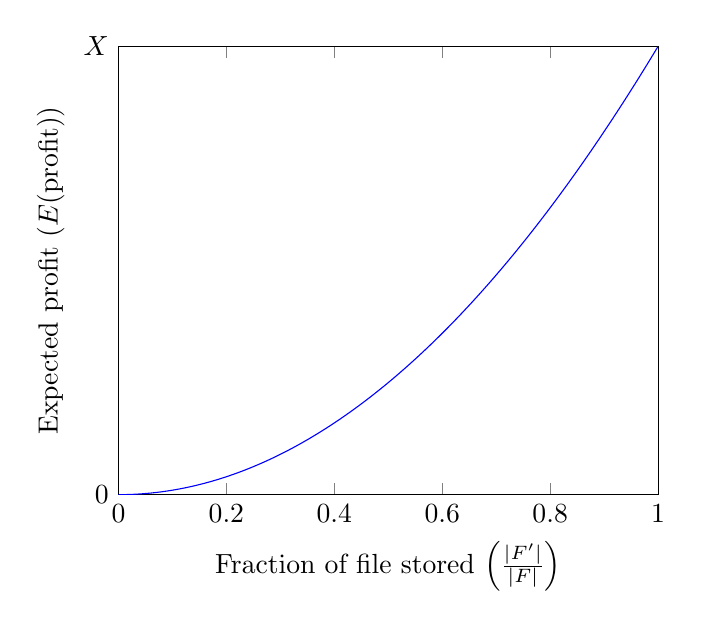
\begin{tikzpicture}
  \begin{axis}[ 
    xmin=0, xmax=1,
    ymin=0, ymax=1,
    xlabel={Fraction of file stored $\left(\frac{|F'|}{|F|}\right)$},
    ylabel={Expected profit ($E(\text{profit})$)},
    ytick={0,1},
    yticklabels={0, $X$},
    domain=0:1,
    samples=50,
  ]
    \addplot[smooth,color=blue,mark={}]{x^2}; 
  \end{axis}
\end{tikzpicture}
\caption[Expected attacker profit: multiple chunk proofs]{Expected profit against proportion of chunks stored for the Multiple chunk proofs extension with $Y = 2$.}
\label{fig:eval-graph-multi}
\end{figure}

\begin{figure}[H]
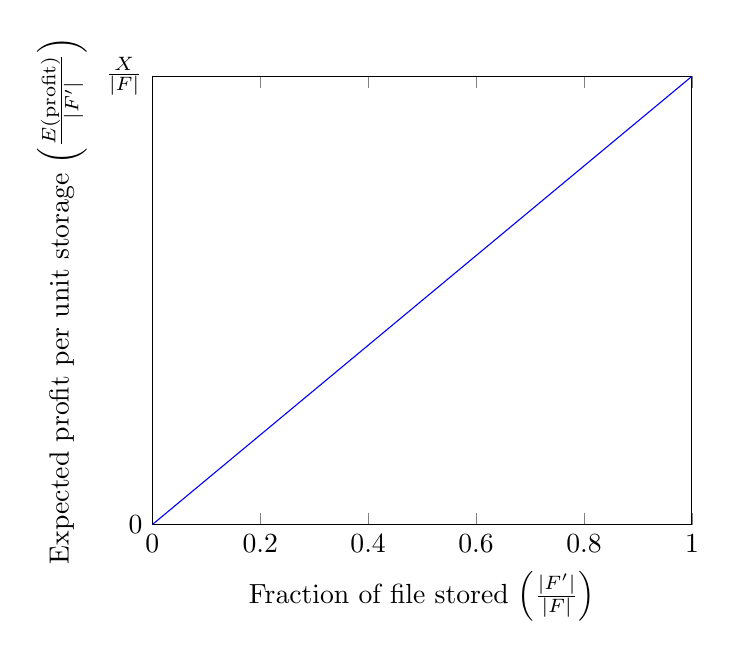
\begin{tikzpicture}
  \begin{axis}[ 
    xmin=0, xmax=1,
    ymin=0, ymax=1,
    xlabel={Fraction of file stored $\left(\frac{|F'|}{|F|}\right)$},
    ylabel={Expected profit per unit storage $\left(\frac{E(\text{profit})}{|F'|}\right)$},
    ytick={0,1},
    yticklabels={0, $\frac{X}{|F|}$},
    domain=0:1,
    samples=50,
  ]
    \addplot[smooth,color=blue,mark={}]{x}; 
  \end{axis}
\end{tikzpicture}
\caption[Expected attacker profit per unit storage: multiple chunk proofs]{Expected profit per unit storage against proportion of chunks stored for the Multiple chunk proofs extension with $Y = 2$.}
\label{fig:eval-graph-multi-storage}
\end{figure}

\subsection{Lock-in}

See section \ref{ext-lockin} for details.

Here the contract is given $X$ Ether by the owner, and $L$ by the locking in storage node.
The locking in storage node is later allowed to submit a valid proof which will return the full $X + L$ as a reward.
\[E(\text{profit}) = (X + L) \cdot \frac{|F'|}{|F|} - L\]
Figures \ref{eval-graph-lockin} and \ref{eval-graph-lockin-storage} show how this encourages nodes to store the whole file.

\begin{figure}[H]
\begin{tikzpicture}
  \begin{axis}[ 
    xmin=0, xmax=1,
    ymin=-2, ymax=1,
    xlabel={Fraction of file stored $\left(\frac{|F'|}{|F|}\right)$},
    ylabel={Expected profit ($E(\text{profit})$)},
    ytick={-2,0,1},
    yticklabels={$-L$, 0, $X$},
    axis lines=middle,
    x label style={at={(axis description cs:1.02,0.6666666)},anchor=west},
    ylabel near ticks,
    domain=0:1,
  ]
    \addplot[color=blue,mark={}]{3*x - 2}; 
  \end{axis}
\end{tikzpicture}
\caption[Expected attacker profit: lock-in]{Expected profit against proportion of chunks stored by actor for the Lock-in extension with $L = 2X$.}
\label{eval-graph-lockin}
\end{figure}

\begin{figure}[H]
\begin{tikzpicture}
  \begin{axis}[ 
    xmin=0, xmax=1,
    ymin=-2, ymax=1,
    xlabel={Fraction of file stored $\left(\frac{|F'|}{|F|}\right)$},
    ylabel={Expected profit per unit storage $\left(\frac{E(\text{profit})}{|F'|}\right)$},
    ytick={-2,0,1},
    yticklabels={$\frac{-L}{|F|}$, 0, $\frac{X}{|F|}$},
    axis lines=middle,
    x label style={at={(axis description cs:1.02,0.6666666)},anchor=west},
    ylabel near ticks,
    domain=0:1,
  ]
    \addplot[color=blue,mark={}]{(3*x - 2)/x}; 
  \end{axis}
\end{tikzpicture}
\caption[Expected attacker profit per unit storage: lock-in]{Expected profit per unit storage against proportion of chunks stored by actor for the Lock-in extension with $L = 2X$.}
\label{eval-graph-lockin-storage}
\end{figure}

%
%\subsection{Multi-chunk proofs} \label{combine-ext}
%
%Here we combine the lock-in extension with multi-chunk proofs.
%This means we require $Y$ proofs for different chunks of $F$, which gives the following expected profit.
%
%\[E(\text{profit}) = (X + L) \cdot \left(\frac{|F'|}{|F|}\right)^Y - L\]
%
%This is a considerable improvement over either extension alone, however it's still possible for an actor to make a  (albeit reduced) profit
%whilst not storing the whole file. It is likely the file will be encrypted and so this may render the entire file lost.
%
%\begin{figure}[H]
%\begin{tikzpicture}
%  \begin{axis}[ 
%    xmin=0, xmax=1,
%    ymin=-2, ymax=1,
%    xlabel={Fraction of file stored $\left(\frac{|F'|}{|F|}\right)$},
%    ylabel={Expected profit ($E(\text{profit})$)},
%    ytick={-2,0.0,1},
%    yticklabels={$-L$, 0, $X$},
%    axis lines=middle,
%    x label style={at={(axis description cs:1.02,0.6666666)},anchor=west},
%    ylabel near ticks,
%    domain=0:1,
%    samples=50,
%  ]
%    \addplot[smooth,color=blue,mark={}]{3*x^2 - 2}; 
%  \end{axis}
%\end{tikzpicture}
%
%\caption[Expected attacker profit: multiple chunk proofs and lock-in]{Expected profit against proportion of chunks stored by actor with both the Lock-in extension and multiple chunk proofs with $L = 2X$ and $Y = 2$.}
%\end{figure}

\subsection{Erasure codes}

Adding an Erasure code allows the file to be recovered even if some chunks are lost or corrupted.
For example, we could add 25\% to the file size to ensure that the file can be recovered even if 20\% (of the now larger file)
is lost.

Combining this with the other extensions in this section allows us to make it unprofitable to not store enough of the file to allow recovery,
as demonstrated in Figure~\ref{eval-graph-erasure}.



\begin{figure}[H]
\begin{tikzpicture}
  \begin{axis}[ 
    xmin=0, xmax=1,
    ymin=-2, ymax=1,
    xlabel={Fraction of file stored $\left(\frac{|F'|}{|F|}\right)$},
    ylabel={Expected profit ($E(\text{profit})$)},
    ytick={-2,0,1},
    yticklabels={$-L$, 0, $X$},
    axis lines=middle,
    x label style={at={(axis description cs:1.02,0.6666666)},anchor=west},
    ylabel near ticks,
    domain=0:1,
    samples=50,
  ]
    \addplot[smooth,color=blue,mark={}]{3*x^2 - 2}; 
    \addplot[color=red,mark=none] coordinates {(0.8, -2) (0.8, 1)};
  \end{axis}
\end{tikzpicture}

\caption[Expected attacker profit: erasure code]{Expected profit against proportion of chunks stored with both the Lock-in extension and multiple chunk proofs with $L = 2X$ and $Y = 2$.
The red line represents the proportion (80\%) of the chunks required to fully reconstruct the original file.}
\label{eval-graph-erasure}
\end{figure}

\subsection{RSA extension}

%Was it successful, limitiations of Ethereum.

\chapter{Conclusion}

I have achieved the original aims set out in the proposal for this project.
I have a working implementation and an analysis of its properties.
I have also completed several extensions and looked at the limitations of the Ethereum network with respect to this project.

The implementation is working and would be practical to use as part of an incentive system for a distributed file system.
An implementation of a secure RSA or Elliptic curve based version is not yet practical is not yet practical for Ethereum,
however the proof of concept gives hope that it will be in the future.

I have enjoyed completing the project and have learnt a lot about Ethereum and its ecosystem.
Whilst planning and implementing the RSA extension I also learnt more about modular arithmetic and group theory than had
anticipated when starting the project.

If I had more time then, once the proposals for RSA and ECC primitives had been deployed I would like to write
a full implementation, possibly as a fork of Swarm.

%Difficult bits





%It worked
%What I would do differently









%%%%%%%%%%%%%%%%%%%%%
%Worth getting better security - probably not, still have to get file back.

\begingroup
%\sloppy
\raggedright
\printbibliography
\endgroup
% If multiple contracts wanted, simply encrypt file with different keys.

\begin{appendices}

\chapter{Proposal}

\includepdf[pages=-]{proposal.pdf}

\chapter{Contract code} \label{app-contract}

\chapter{Java proof generation} \label{app-java}

\chapter{Optimal chunk length} \label{app-chunk-size}

Recall section~\ref{chunk-size-proof-size}.
The size of the proof is:
\[|r| = c + 32 \cdot \left\lceil\log_2\left(\frac{|F|}{c}\right)\right\rceil\]
which can only be minimal when $\frac{|F|}{c}$ is a power of 2 (otherwise we can decrease $c$ and hence $|r|$ with no change in the log term).

We have $\frac{|F|}{c} = 2^n$ for some $n \in \mathbb{N}$, so we re-express $|r|$ in terms of $n$.
\[|r| = \frac{|F|}{2^n} + 32 n\]

We attempt to find the minimum, letting $n$ be in $\mathbb{R}$ for now.
\begin{align*}
\frac{d |r|}{d n} = 0 &\implies 32 - \ln(2) \cdot |F| \cdot 2^{-n} = 0\\
&\implies n = \log_2(|F|) - 5 + \log_2(\ln(2))
\end{align*}

An algorithm for computing the optimal chunk size follows from this
\begin{enumerate}
\item Compute the two natural numbers $n_1, n_2$ closest to $\log_2(|F|) - 5 + \log_2(\ln(2))$.
\item Let $c_i = \left\lceil \frac{|F|}{2^{n_i}}\right\rceil$.
\item Take $j \in \{1, 2\}$ such that $c_j + 32 \cdot \log\left(\frac{|F|}{c_j}\right)$ is minimized.
\item $c = c_j$.
\end{enumerate}
\end{appendices}
\end{document}
